\section{Wstęp}
\subsection{Cel projektu}
Celem projektu jest wybranie struktury modeli oraz ich identyfikacja na podstawie zebranego zestawu danych. Pierwszy zestaw zawiera pomiary statyki obiektu, drugi natomiast - pomiary jego dynamiki.
\subsection{Wizualizacja danych}
\subsubsection{Dane do modelu statycznego}
Dane potrzebne do wyznaczenia modelu statycznego zostały pobrane z pliku $danestat4.txt$. Zawarte w nim punty zostały przedstawione na wykresie poniżej.
\begin{figure}[H]
\centering
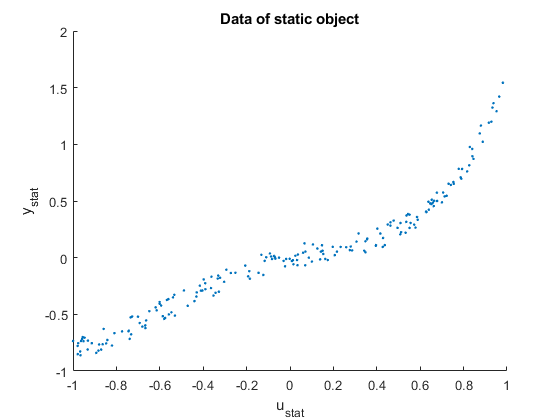
\includegraphics[width=15cm]{images/21.png}
\caption{Zbiór danych wykorzystany do wyznaczenia modelu statycznego.}
\label{fig:1}
\end{figure}
W celu wyznaczenia modelu należało przygotować dane, dzieląc go odpowiednio na zbiór uczący oraz weryfikujący. Przyjęto, że zbiór uczący będzie stanowił 30$\%$ całej bazy danych, natomiast zbiór weryfikujący - pozostałe 70$\%$. Wynik podziału został przedstawiony na wykresie poniżej. Jak widać, zarówno zbiór uczący, jak i weryfikujący, zawierają próbki z prawie całej dziedziny (-1;1).
\begin{figure}[H]
\centering
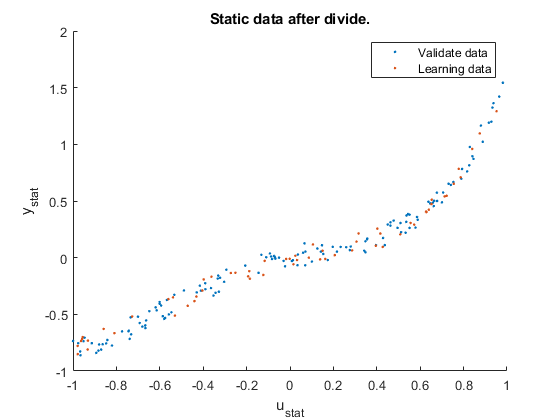
\includegraphics[width=15cm]{images/25.png}
\caption{Zbiór danych wykorzystany do wyznaczenia modelu statycznego po podziale.}
\label{fig:1}
\end{figure}
\subsubsection{Model dynamiczny}
Dane do przygotowania oraz weryfikacji modelu dynamicznego zawarte zostały w plikach $danedynucz4.txt$ oraz $danedynwer4.txt$. Dane zostały już wcześniej podzielone, więc nie było potrzeby ich dzielenia.Każdy ze zbiorów posiada po 2000 próbek.\\
Zbiory uczący oraz weryfikujący zaprezentowano na wykresach poniżej.
\begin{figure}[H]
\centering
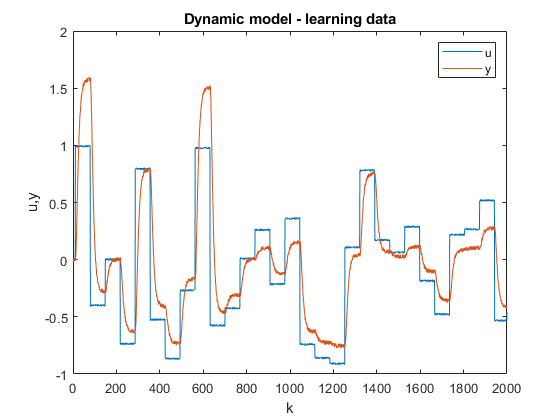
\includegraphics[width=15cm]{images/23.png}
\caption{Dane uczące do modelu dynamicznego.}
\label{fig:2}
\end{figure}
\begin{figure}[H]
\centering
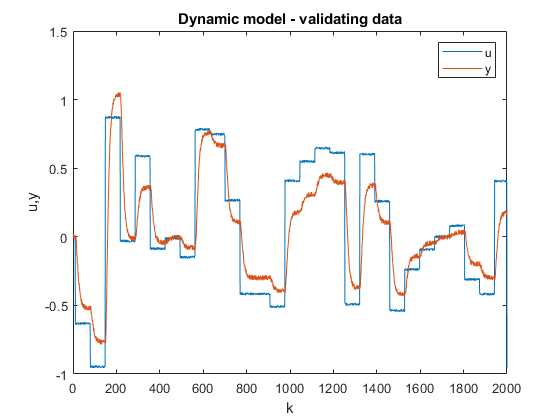
\includegraphics[width=15cm]{images/24.png}
\caption{Dane weryfikujące do modelu dynamicznego.}
\label{fig:3}
\end{figure}
\section{Identyfikacja modeli statycznych}
W tej sekcji przedstawione zostały wyniki tworzenia modeli statycznych o strukturze:
\begin{equation}
y(u)=a_{0}+\sum_{i=1}^{N}a_{i}u^{i}
\end{equation}
gdzie:
\begin{itemize}
\item N - stopień wielomianu modelu,
\item a - współczynniki modelu.
\end{itemize}
Model liniowy jest szczególnym przypadkiem modelu wielomianowego (o 1. stopniu), więc został on omówiony razem z modelami o wyższych stopniach.
\subsection{Zestawienie otrzymanych modeli}
\begin{table}[H]
\centering
\begin{tabular}{|c|c|c|c|}
\hline
St. Wielomianu & Ilość wsp. & $E_{learning}$ & $E_{ver}$ \\ \hline
1              & 2             & 0.016835              & 0.026768         \\ \hline
2              & 3             & 0.013875              & 0.021407         \\ \hline
3              & 4             & 0.005283              & 0.009850         \\ \hline
4              & 5             & 0.002789              & 0.003813         \\ \hline
5              & 6             & 0.002754              & 0.004035         \\ \hline
6              & 7             & 0.002683              & 0.004457         \\ \hline
\end{tabular}
\caption{Zestawienie modeli statycznych otrzymanych metodą najmniejszych kwadratów.}
\end{table}
\begin{figure}[H]
\centering
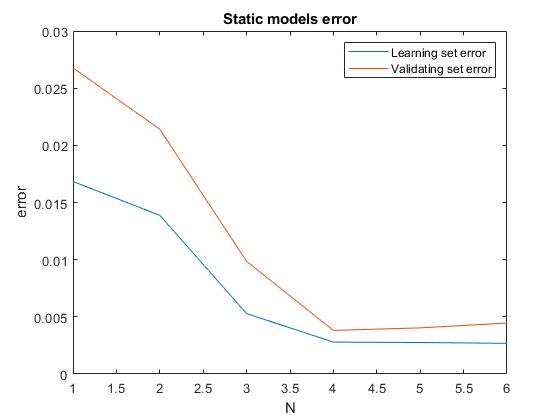
\includegraphics[width=15cm]{images/s_error.png}
\caption{Przebieg wartości błędów modelowania od stopnia modelu.}
\label{fig:s_error}
\end{figure}
\subsection{Wizualna ocena otrzymanych modeli}
\begin{figure}[H]
\centering
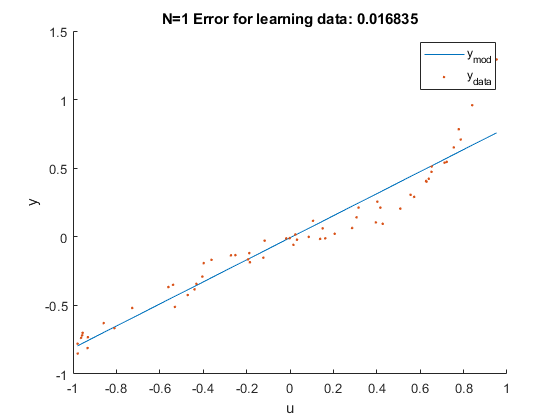
\includegraphics[width=15cm]{images/s1.png}
\caption{Porównanie modelu statycznego 1. rzędu z danymi uczącymi.}
\label{fig:s1}
\end{figure}
\begin{figure}[H]
\centering
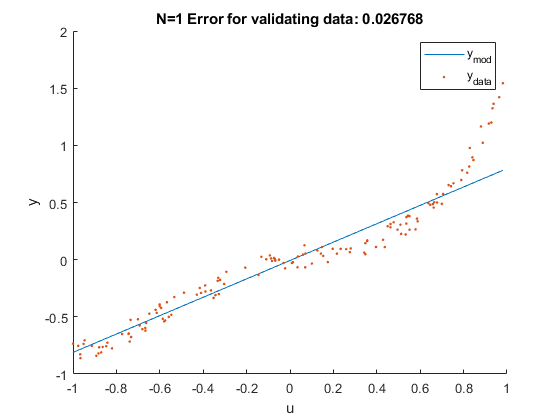
\includegraphics[width=15cm]{images/s2.png}
\caption{Porównanie modelu statycznego 1. rzędu z danymi weryfikującymi.}
\label{fig:s2}
\end{figure}
\begin{figure}[H]
\centering
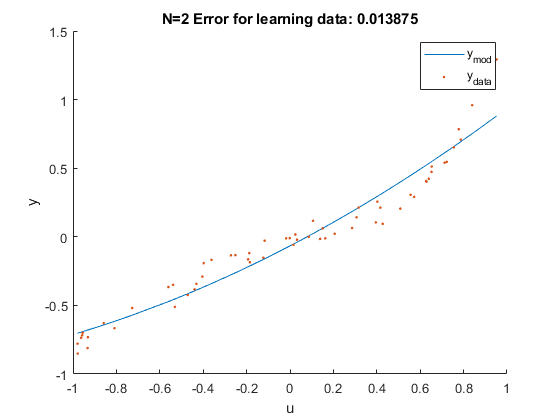
\includegraphics[width=15cm]{images/s3.png}
\caption{Porównanie modelu statycznego 2. rzędu z danymi uczącymi.}
\label{fig:s3}
\end{figure}
\begin{figure}[H]
\centering
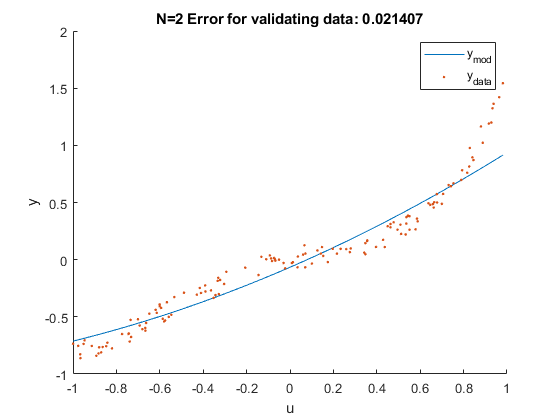
\includegraphics[width=15cm]{images/s4.png}
\caption{Porównanie modelu statycznego 2. rzędu z danymi weryfikującymi.}
\label{fig:s4}
\end{figure}
\begin{figure}[H]
\centering
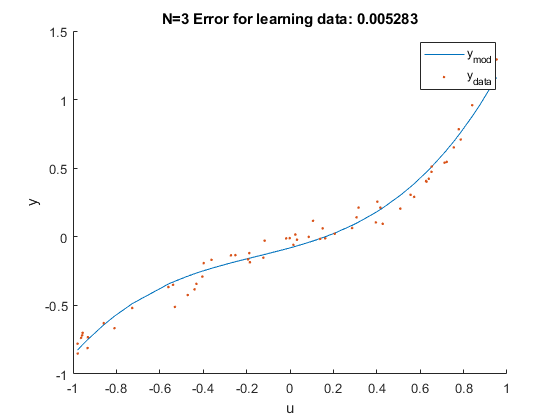
\includegraphics[width=15cm]{images/s5.png}
\caption{Porównanie modelu statycznego 3. rzędu z danymi uczącymi.}
\label{fig:s5}
\end{figure}
\begin{figure}[H]
\centering
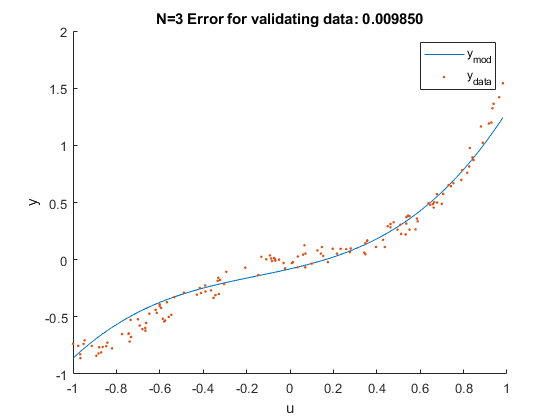
\includegraphics[width=15cm]{images/s6.png}
\caption{Porównanie modelu statycznego 3. rzędu z danymi weryfikującymi.}
\label{fig:s6}
\end{figure}
\begin{figure}[H]
\centering
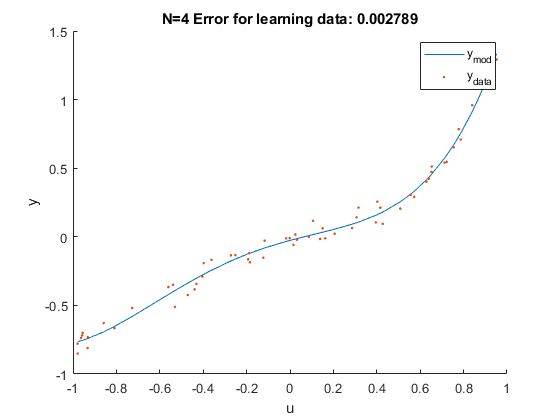
\includegraphics[width=15cm]{images/s7.png}
\caption{Porównanie modelu statycznego 4. rzędu z danymi uczącymi.}
\label{fig:s7}
\end{figure}
\begin{figure}[H]
\centering
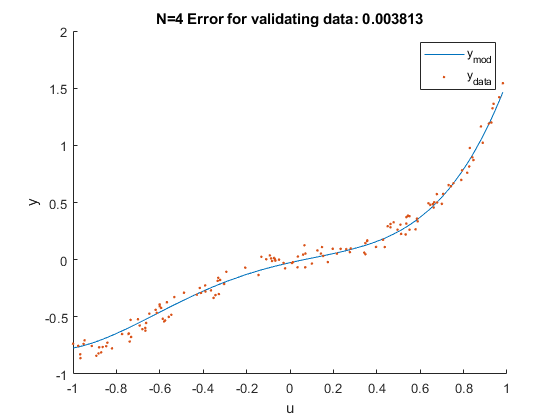
\includegraphics[width=15cm]{images/s8.png}
\caption{Porównanie modelu statycznego 4. rzędu z danymi weryfikującymi.}
\label{fig:s8}
\end{figure}
\begin{figure}[H]
\centering
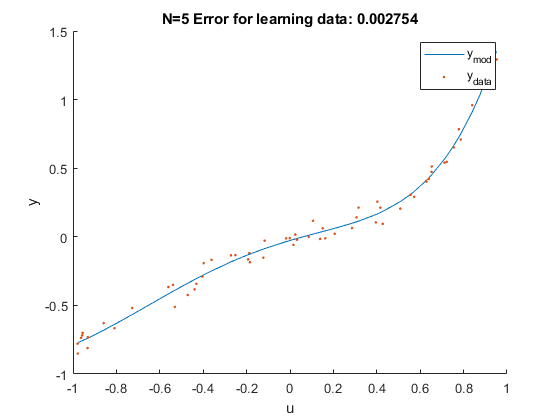
\includegraphics[width=15cm]{images/s9.png}
\caption{Porównanie modelu statycznego 5. rzędu z danymi uczącymi.}
\label{fig:s9}
\end{figure}
\begin{figure}[H]
\centering
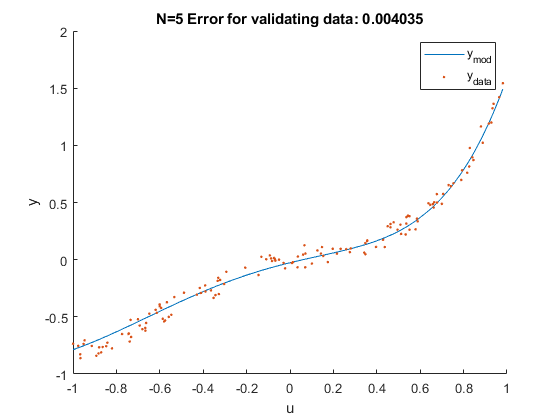
\includegraphics[width=15cm]{images/s10.png}
\caption{Porównanie modelu statycznego 5. rzędu z danymi weryfikującymi.}
\label{fig:s10}
\end{figure}
\begin{figure}[H]
\centering
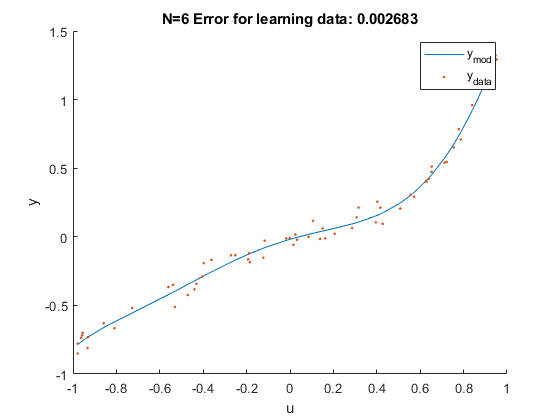
\includegraphics[width=15cm]{images/s11.png}
\caption{Porównanie modelu statycznego 6. rzędu z danymi uczącymi.}
\label{fig:s11}
\end{figure}
\begin{figure}[H]
\centering
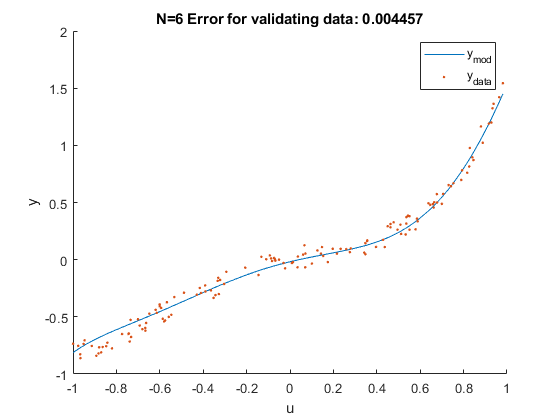
\includegraphics[width=15cm]{images/s12.png}
\caption{Porównanie modelu statycznego 6. rzędu z danymi weryfikującymi.}
\label{fig:s12}
\end{figure}
\subsection{Podsumowanie}
Jako najlepszy model wybrany został model o 4. stopniu wielomianu. Jest to model o najwyższym stopniu, dla którego obserwujemy malejące wartości błędu dla zbioru weryfikującego, to znaczy, że wszystkie modele wyższego stopnia są przewymiarowane, przez co zbytnio dopasowują się do danych zawartych w zbiorze uczącym. Ponadto, pod względem wizualnym, przebiegi modeli powyżej 4. stopnia nie różnią się znacząco między sobą, więc ograniczenie złożoności modelu do 4. stopnia jest wskazane.
\newpage
\section{Identyfikacja modeli dynamicznych}
W tej sekcji przedstawione zostały wyniki tworzenia modeli dynamicznych o strukturze:
\begin{equation}
y(u)=\sum_{d=1}^{D}\left(\sum_{i=1}^{n_{b}}b_{id}u^d(k-i)+\sum_{i=1}^{n_{a}}a_{id}y^{d}(k-i)\right)
\end{equation}
gdzie:
\begin{itemize}
\item N - stopień wielomianu modelu,
\item a - współczynniki modelu związane z poprzednimi wartościami y,
\item b - współczynniki modelu związane z poprzednimi sterowaniami,
\item D - rząd dynamiki modelu
\end{itemize}
W celu generowania modeli dynamicznych napisany skrypt, który pozwala generować model o dowolnym rozmiarze $n_{a}$, $n_{b}$ oraz stopniu wielomianu. Nie uwzględniano modeli o wyrazach mieszanych. W ostatecznych wynikach, wzięto pod uwagę modele, dla których dynamicza zarówno wejścia, jak i sprzężenia zwrotnego, jest tego samego rzędu ($n_{a}=n_{b}$).
\subsection{Zestawienie otrzymanych modeli}
\begin{table}[H]
\centering
\begin{tabular}{|c|c|c|c|c|c|c|}
\hline
\multicolumn{3}{|c|}{Rząd modelu}                      & \multicolumn{2}{c|}{ARX}   & \multicolumn{2}{c|}{OE}    \\ \hline
Rząd wielomianu & Rząd dynamiki & Ilość wsp. & $E_{learning}$ & $E_{ver}$ & $E_{learning}$ & $E_{ver}$ \\ \hline
1               & 1             &  2                  & 4.0708e-04              & 0.4362         & 0.0443              & 0.5811         \\ \hline
1               & 2             &  4                  & 3.8912e-04              & 0.4363         & 0.0416              & 0.5769         \\ \hline
1               & 3             &  6                  & 3.3780e-04              & 0.4348         & 0.0373              & 0.5667         \\ \hline
2               & 1             &  4                  & 3.5624e-04              & 0.4341         & 0.0177              & 0.5388         \\ \hline
2               & 2             &  8                  & 3.0834e-04              & 0.4340         & 0.0176              & 0.5221         \\ \hline
2               & 3             &  12                & 2.8132e-04              & 0.4336         & 0.0168              & 0.5113         \\ \hline
3               & 1             &  6                  & 3.3404e-04              & 0.4321         & 0.0061              & 0.4654         \\ \hline
3               & 2             &  12                & 2.7043e-04              & 0.4320         & 0.0039              & 0.4616         \\ \hline
3               & 3             &  18                & 2.3980e-04              & 0.4319         & 0.0029              & 0.4585         \\ \hline
4               & 1             &  8                  & 3.2331e-04              & 0.4314         & 0.0031              & 0.4438         \\ \hline
4               & 2             &  16                & 2.5202e-04              & 0.4313         & 0.0019              & 0.4393         \\ \hline
4               & 3             &  2                  & 2.2530e-04              & 0.4313         & 0.0013              & 0.4369         \\ \hline
5               & 1             &  5                  & 3.2286e-04              & 0.4314         & 0.0030              & 0.4466        \\ \hline
5               & 2             &  20                & 2.5090e-04              & 0.4314         & 0.0018              & 0.4434         \\ \hline
5               & 3             &  30                 & 2.2308e-04              & 0.4313         & 0.0011              & 0.4390         \\ \hline
\end{tabular}
\caption{Zestawienie modeli dynamicznych otrzymanych metodą najmniejszych kwadratów.}
\end{table}
Poniżej przedstawiono również wykresy przedstawiające wartości poszczególnych błędów (aby poprawić wrażenia wizualne - również dla modeli nie uwzględnionych w powyższej tabeli).
\begin{figure}[H]
\centering
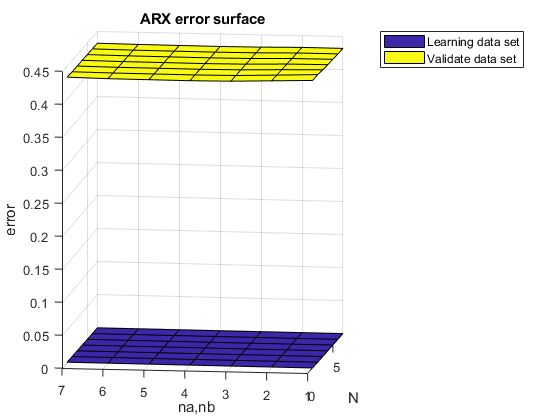
\includegraphics[width=15cm]{images/d_error_arx_ex.png}
\caption{Wykresy błędów wybranych modeli dla pracy w trybie bez rekurencji.}
\label{fig:d_error_arx_ex}
\end{figure}
\begin{figure}[H]
\centering
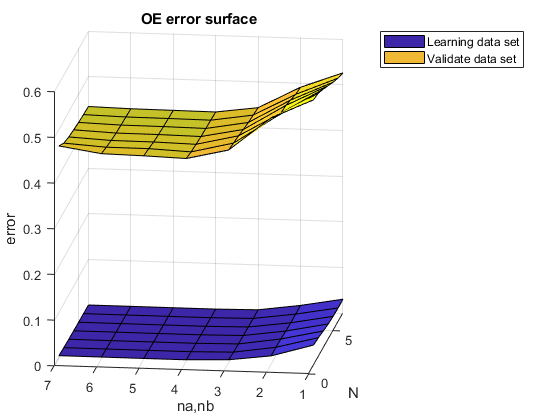
\includegraphics[width=15cm]{images/d_error_oe_ex.png}
\caption{Wykresy błędów wybranych modeli dla pracy w trybie z rekurencją.}
\label{fig:d_error_oe_ex}
\end{figure}
\subsection{Wizualna ocena otrzymanych modeli}
W opisie modeli przyjęto oznaczenia, które jednoznacznie identyfikują model wypisując jego wartości charakterystyczne, czyli $[n_{a},n_{b},stopień]$. Na przykład model drugiego rzędu oraz stopiu wielomianu równym 3, będzie oznaczony $[2,2,3]$.
\subsubsection{Modele z wielomianem 1. stopnia}
\begin{figure}[H]
\centering
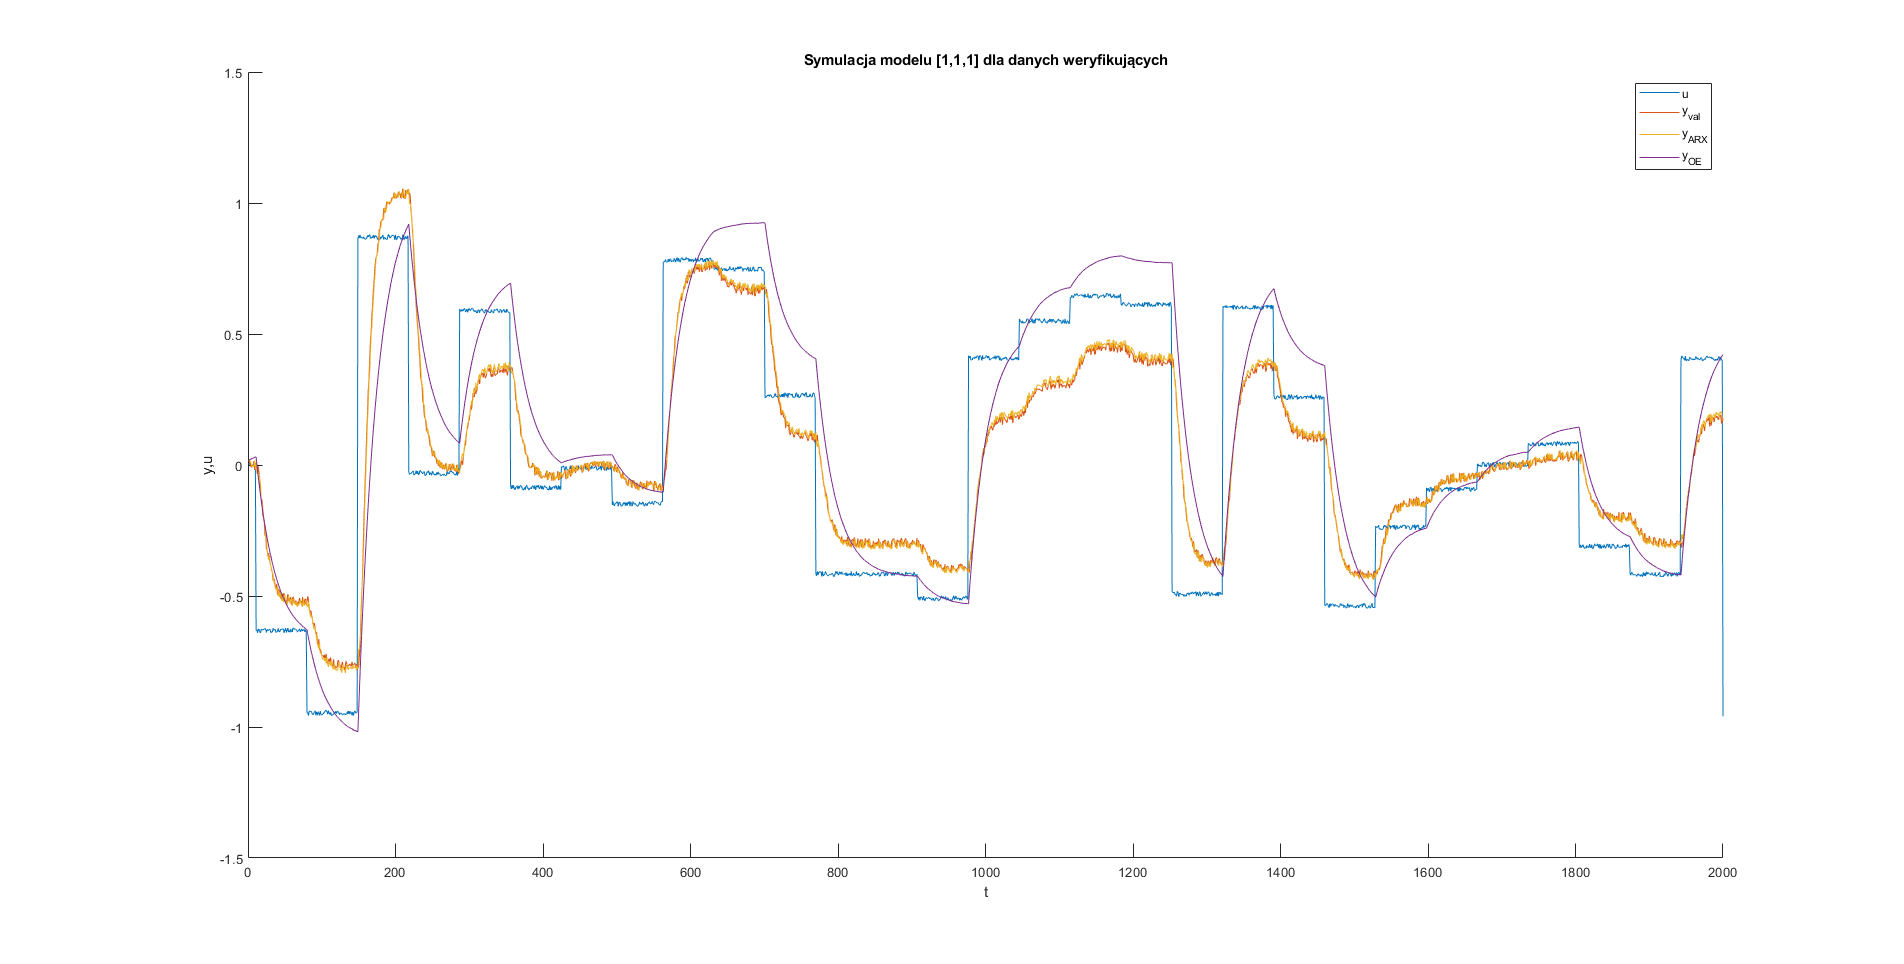
\includegraphics[width=16cm,trim={5cm 1cm 5cm 1cm},clip]{images/d1.png}
\caption{Działanie modelu dynamicznego o 1. stopniu wielomianu i rzędowi dynamiki 1. dla zbioru weryfikującego.}
\label{fig:d1}
\end{figure}
\begin{figure}[H]
\centering
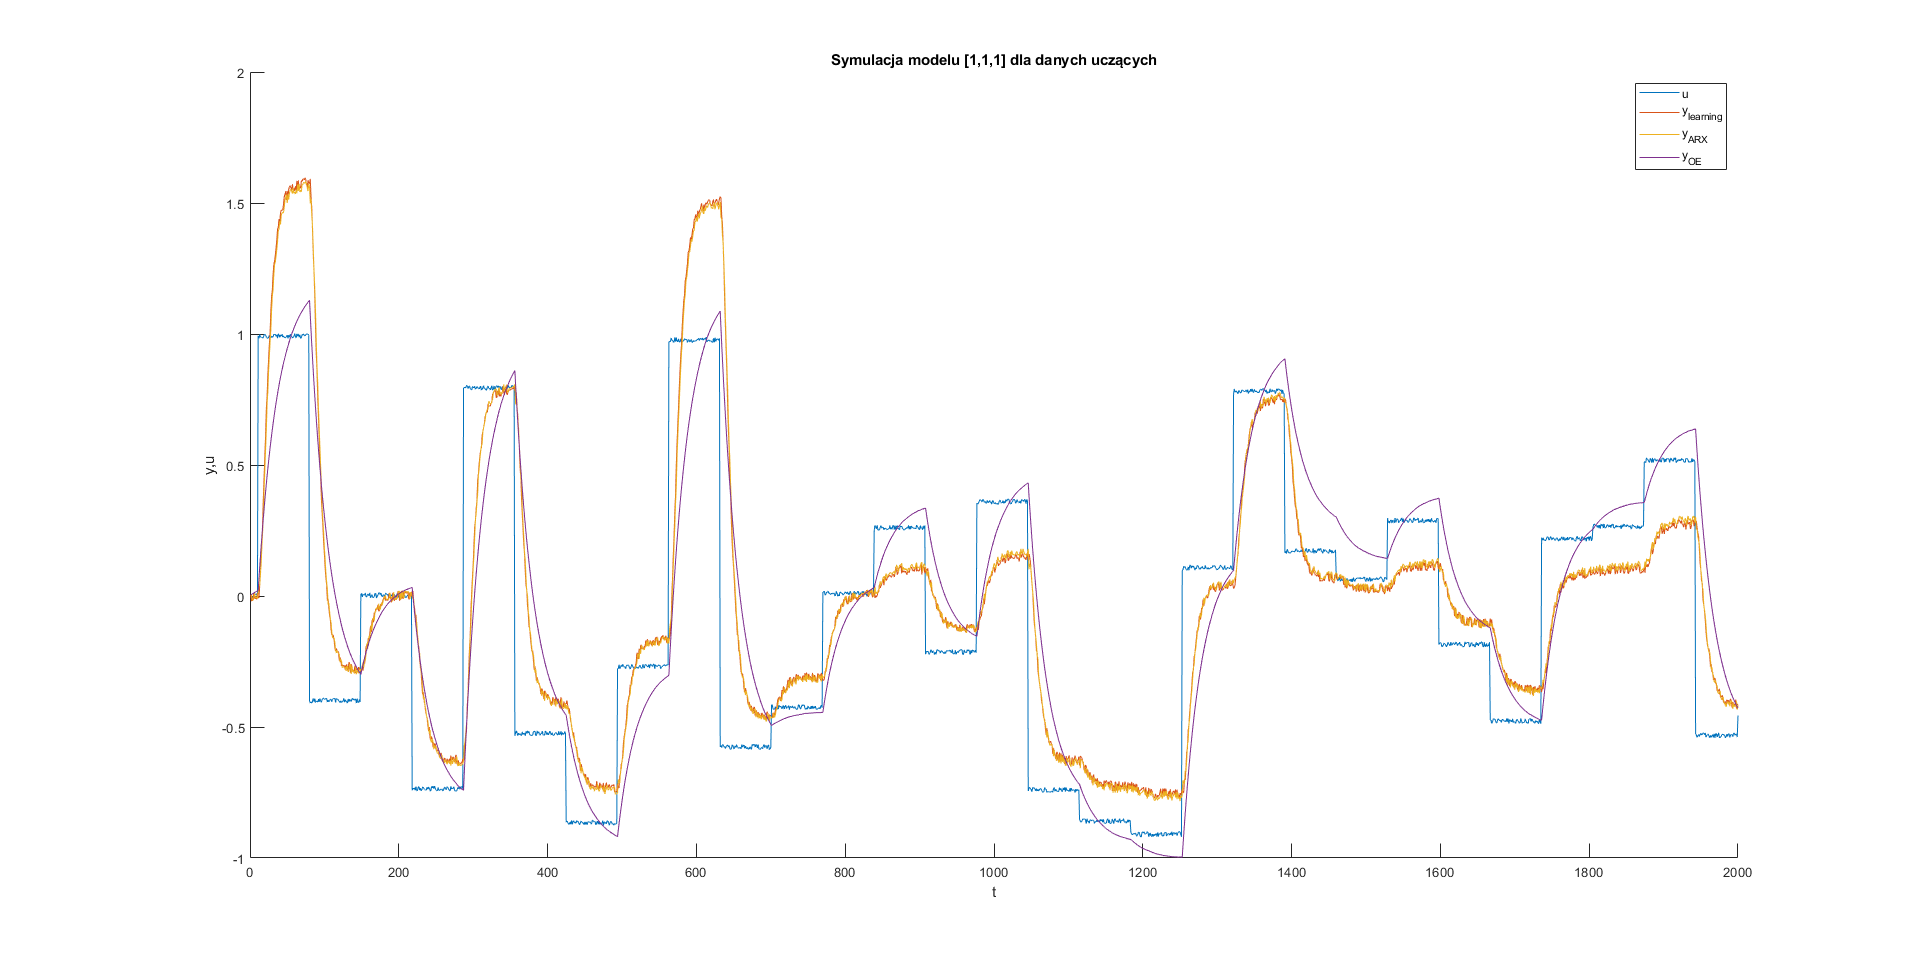
\includegraphics[width=16cm,trim={5cm 1cm 5cm 1cm},clip]{images/d2.png}
\caption{Działanie modelu dynamicznego o 1. stopniu wielomianu i rzędowi dynamiki 1. dla zbioru uczącego.}
\label{fig:d2}
\end{figure}
\begin{figure}[H]
\centering
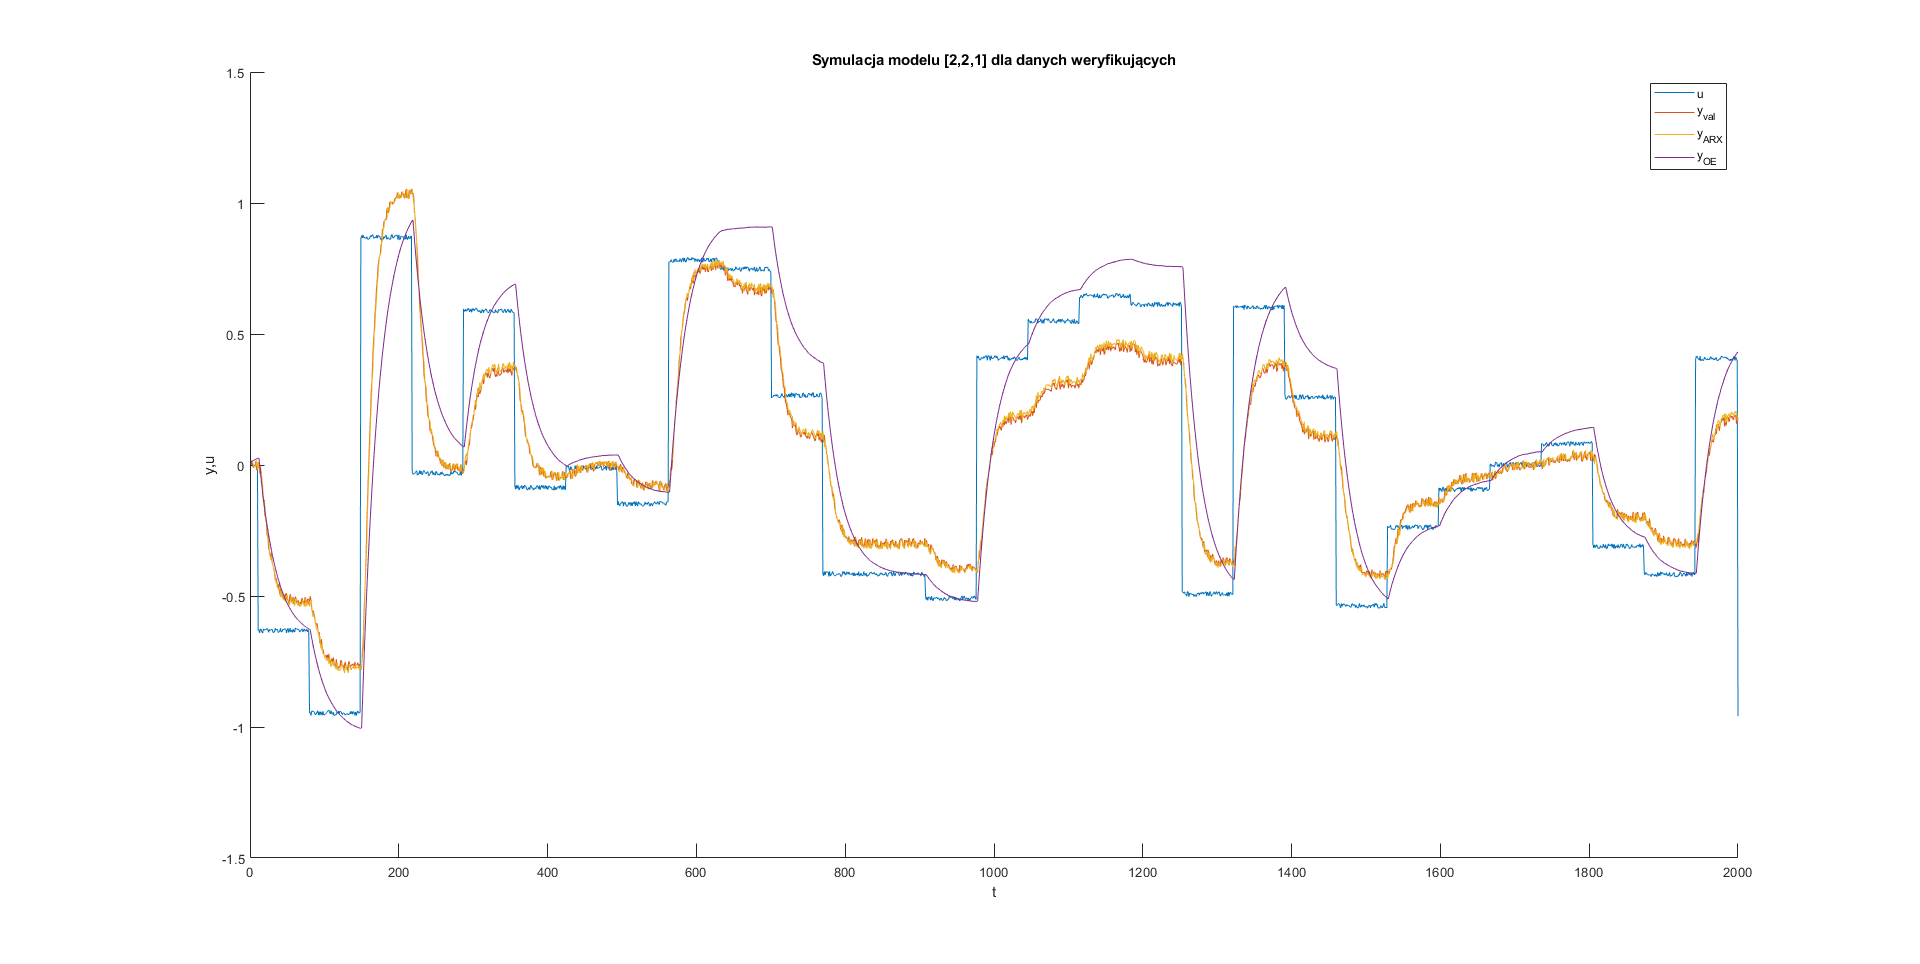
\includegraphics[width=16cm,trim={5cm 1cm 5cm 1cm},clip]{images/d3.png}
\caption{Działanie modelu dynamicznego o 1. stopniu wielomianu i rzędowi dynamiki 2. dla zbioru weryfikującego.}
\label{fig:d3}
\end{figure}
\begin{figure}[H]
\centering
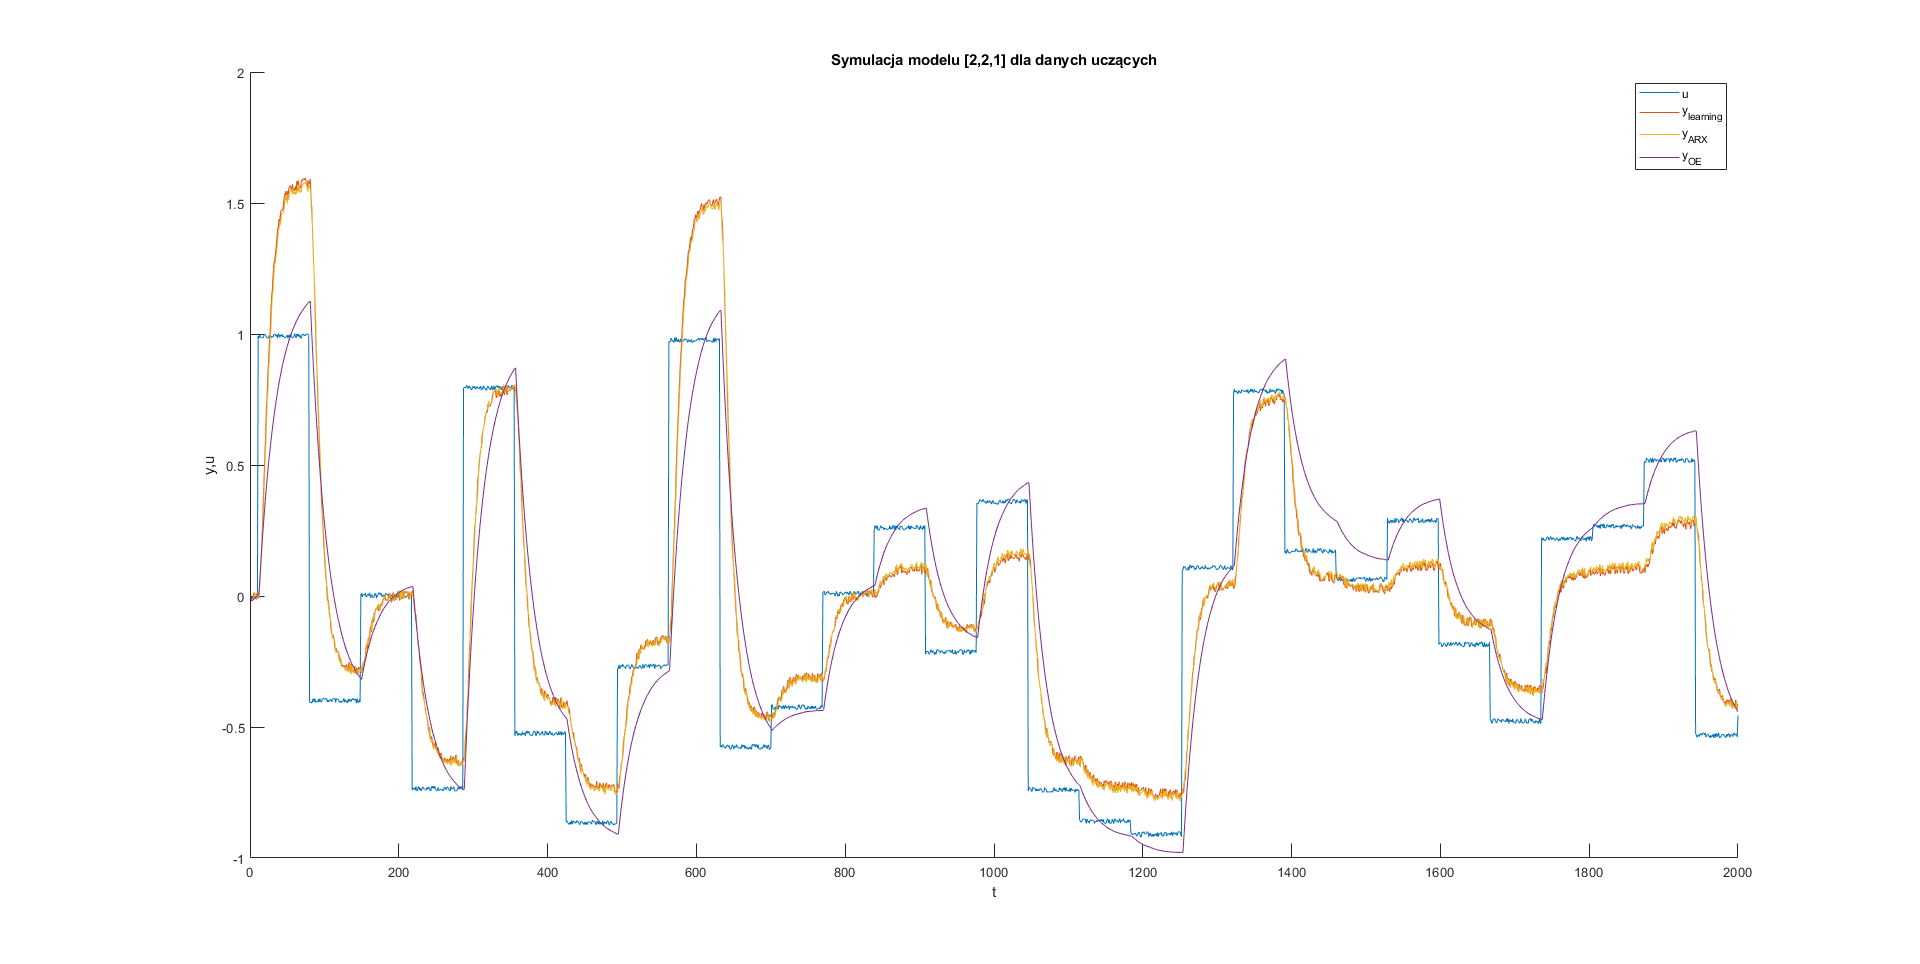
\includegraphics[width=16cm,trim={5cm 1cm 5cm 1cm},clip]{images/d4.png}
\caption{Działanie modelu dynamicznego o 1. stopniu wielomianu i rzędowi dynamiki 2. dla zbioru uczącego.}
\label{fig:d4}
\end{figure}
\begin{figure}[H]
\centering
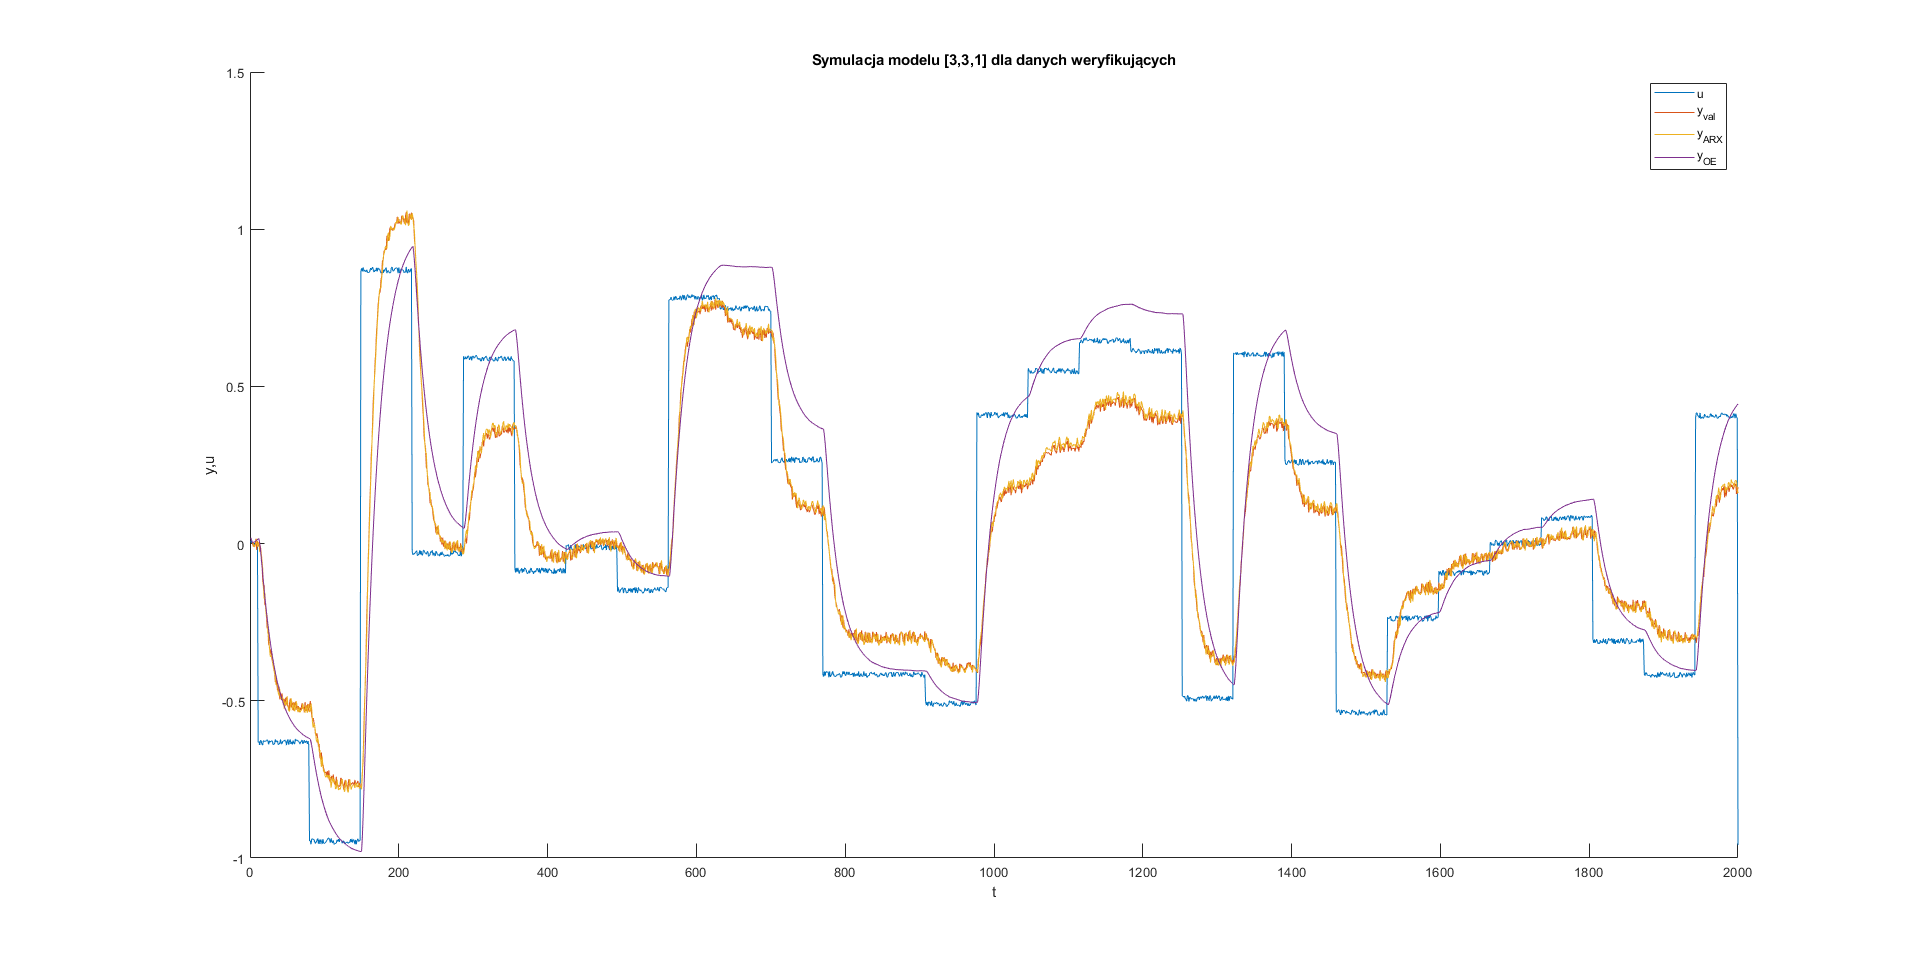
\includegraphics[width=16cm,trim={5cm 1cm 5cm 1cm},clip]{images/d5.png}
\caption{Działanie modelu dynamicznego o 1. stopniu wielomianu i rzędowi dynamiki 3. dla zbioru weryfikującego.}
\label{fig:d5}
\end{figure}
\begin{figure}[H]
\centering
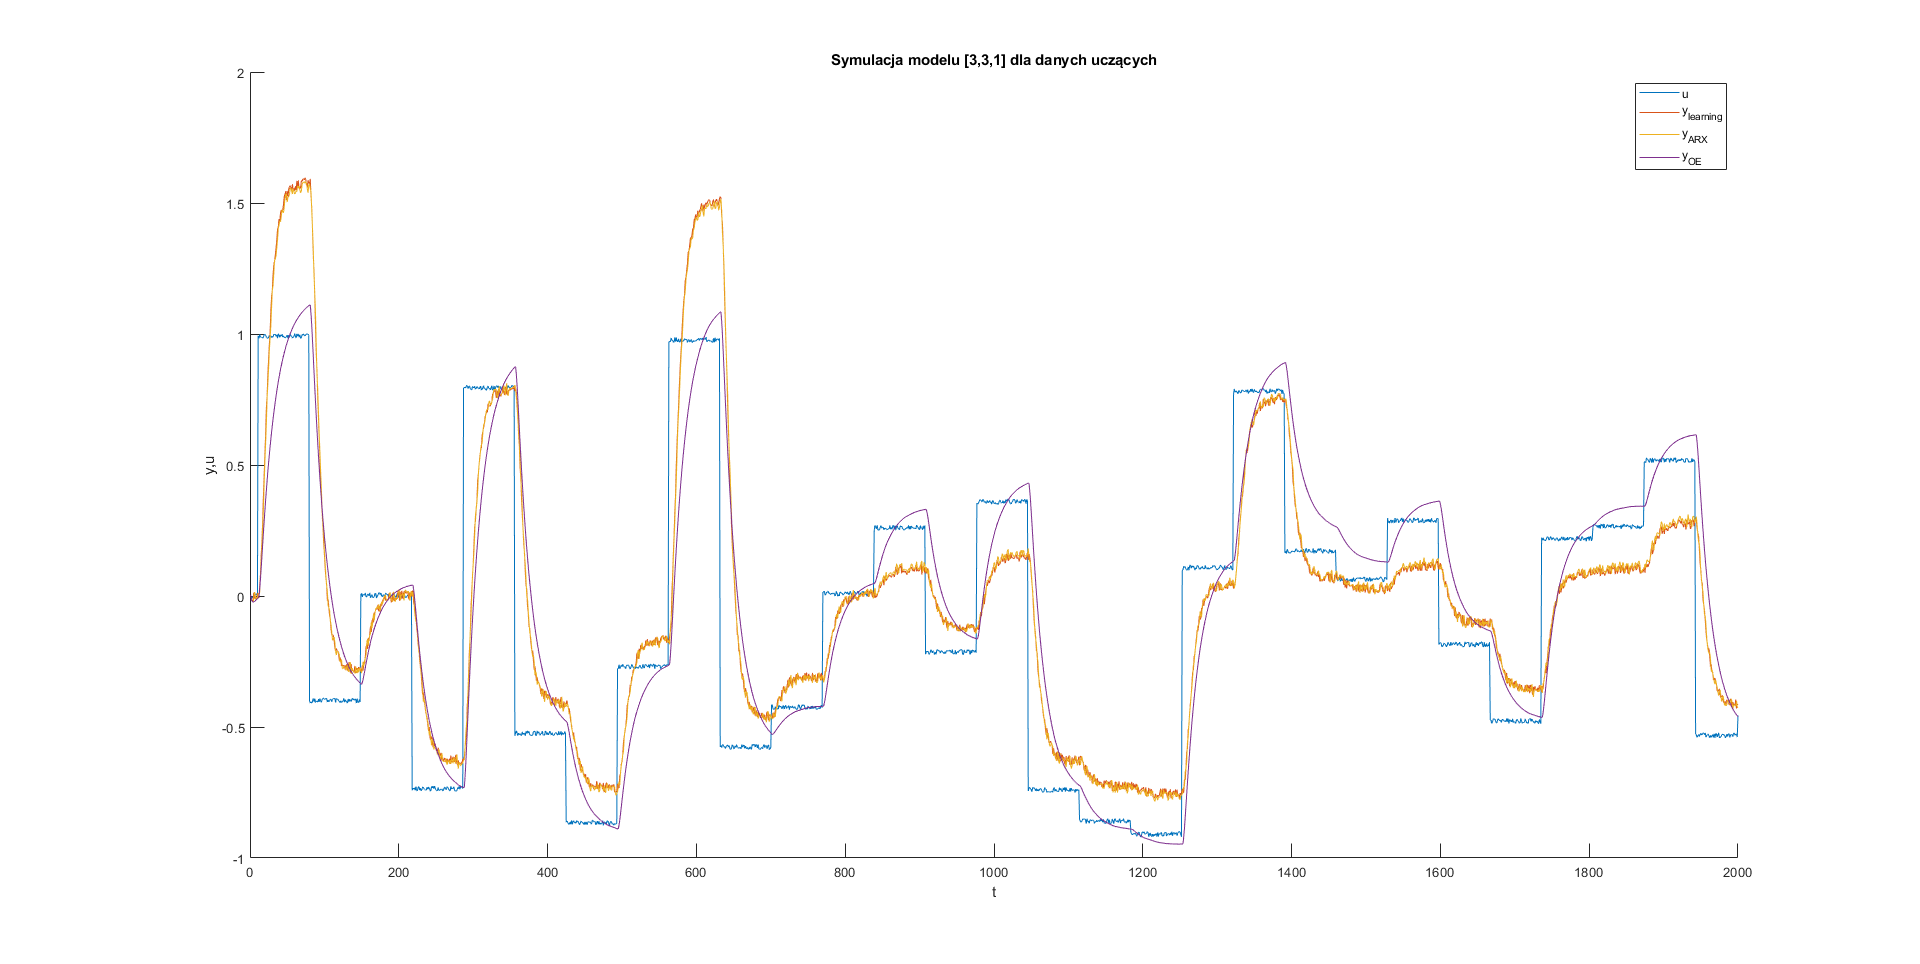
\includegraphics[width=16cm,trim={5cm 1cm 5cm 1cm},clip]{images/d6.png}
\caption{Działanie modelu dynamicznego o 1. stopniu wielomianu i rzędowi dynamiki 3. dla zbioru uczącego.}
\label{fig:d6}
\end{figure}
\subsubsection{Modele z wielomianem 2. stopnia}
\begin{figure}[H]
\centering
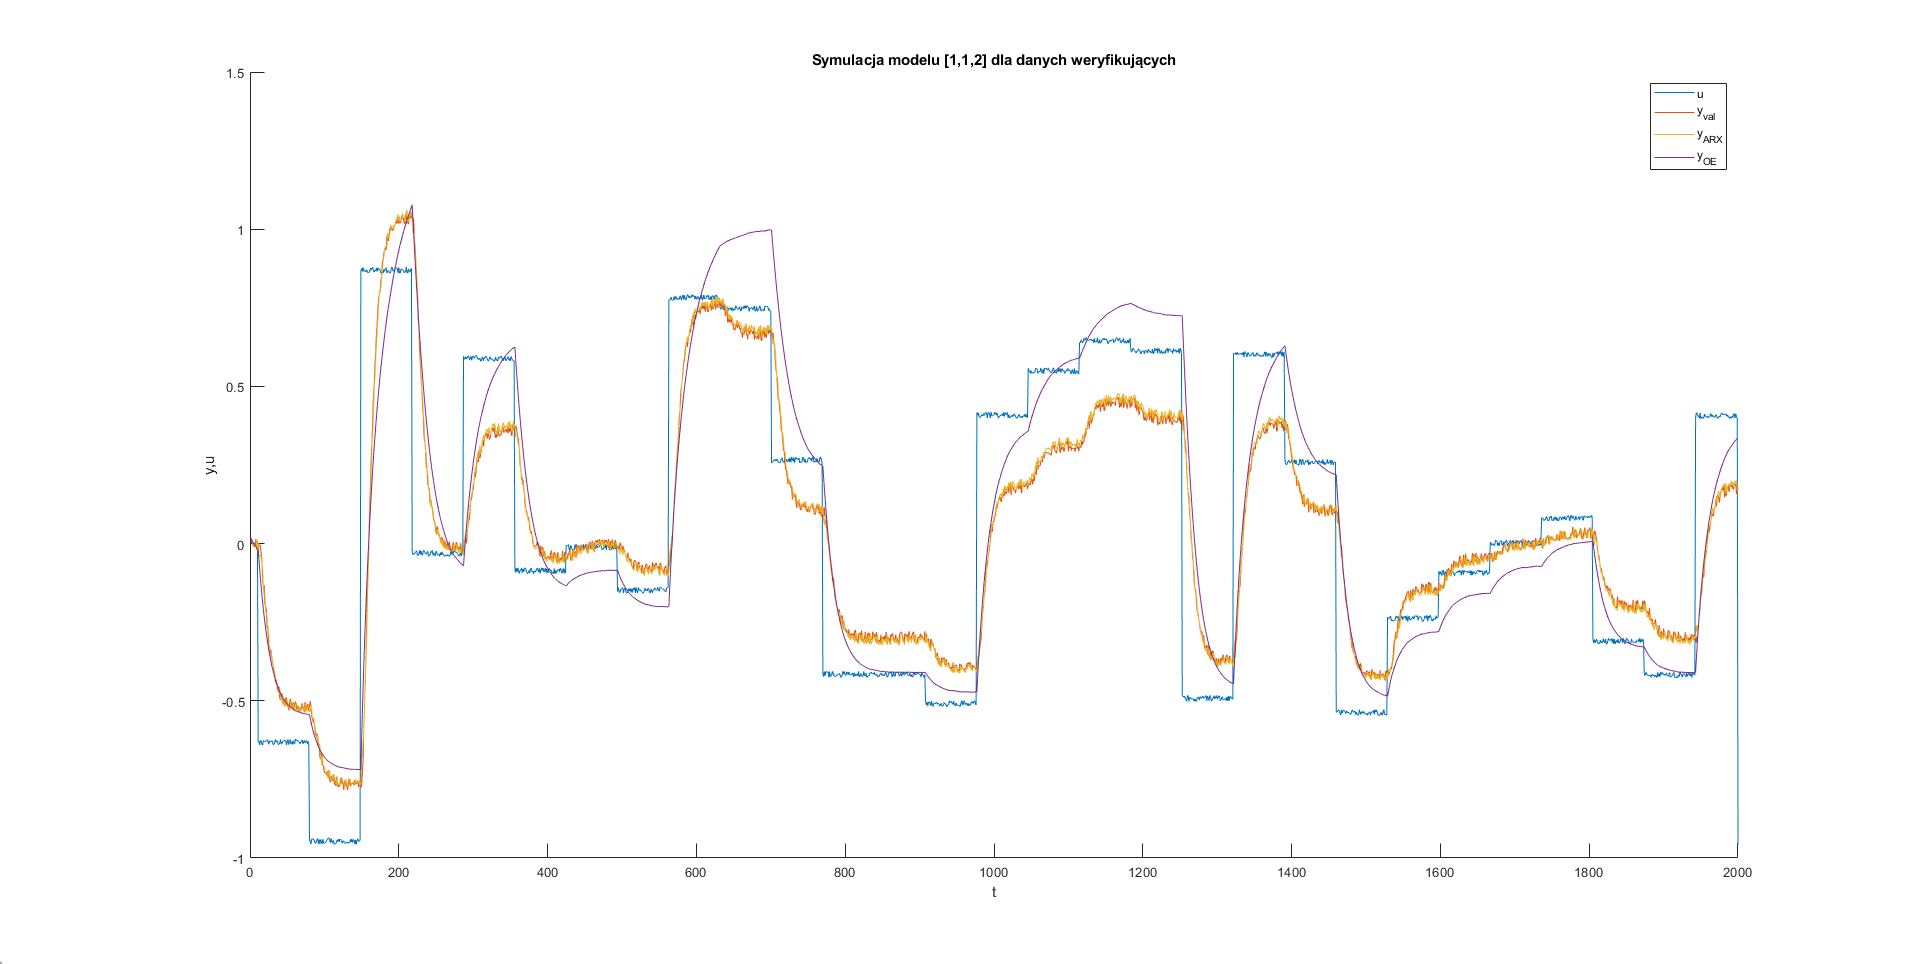
\includegraphics[width=16cm,trim={5cm 1cm 5cm 1cm},clip]{images/d7.png}
\caption{Działanie modelu dynamicznego o 2. stopniu wielomianu i rzędowi dynamiki 1. dla zbioru weryfikującego.}
\label{fig:d7}
\end{figure}
\begin{figure}[H]
\centering
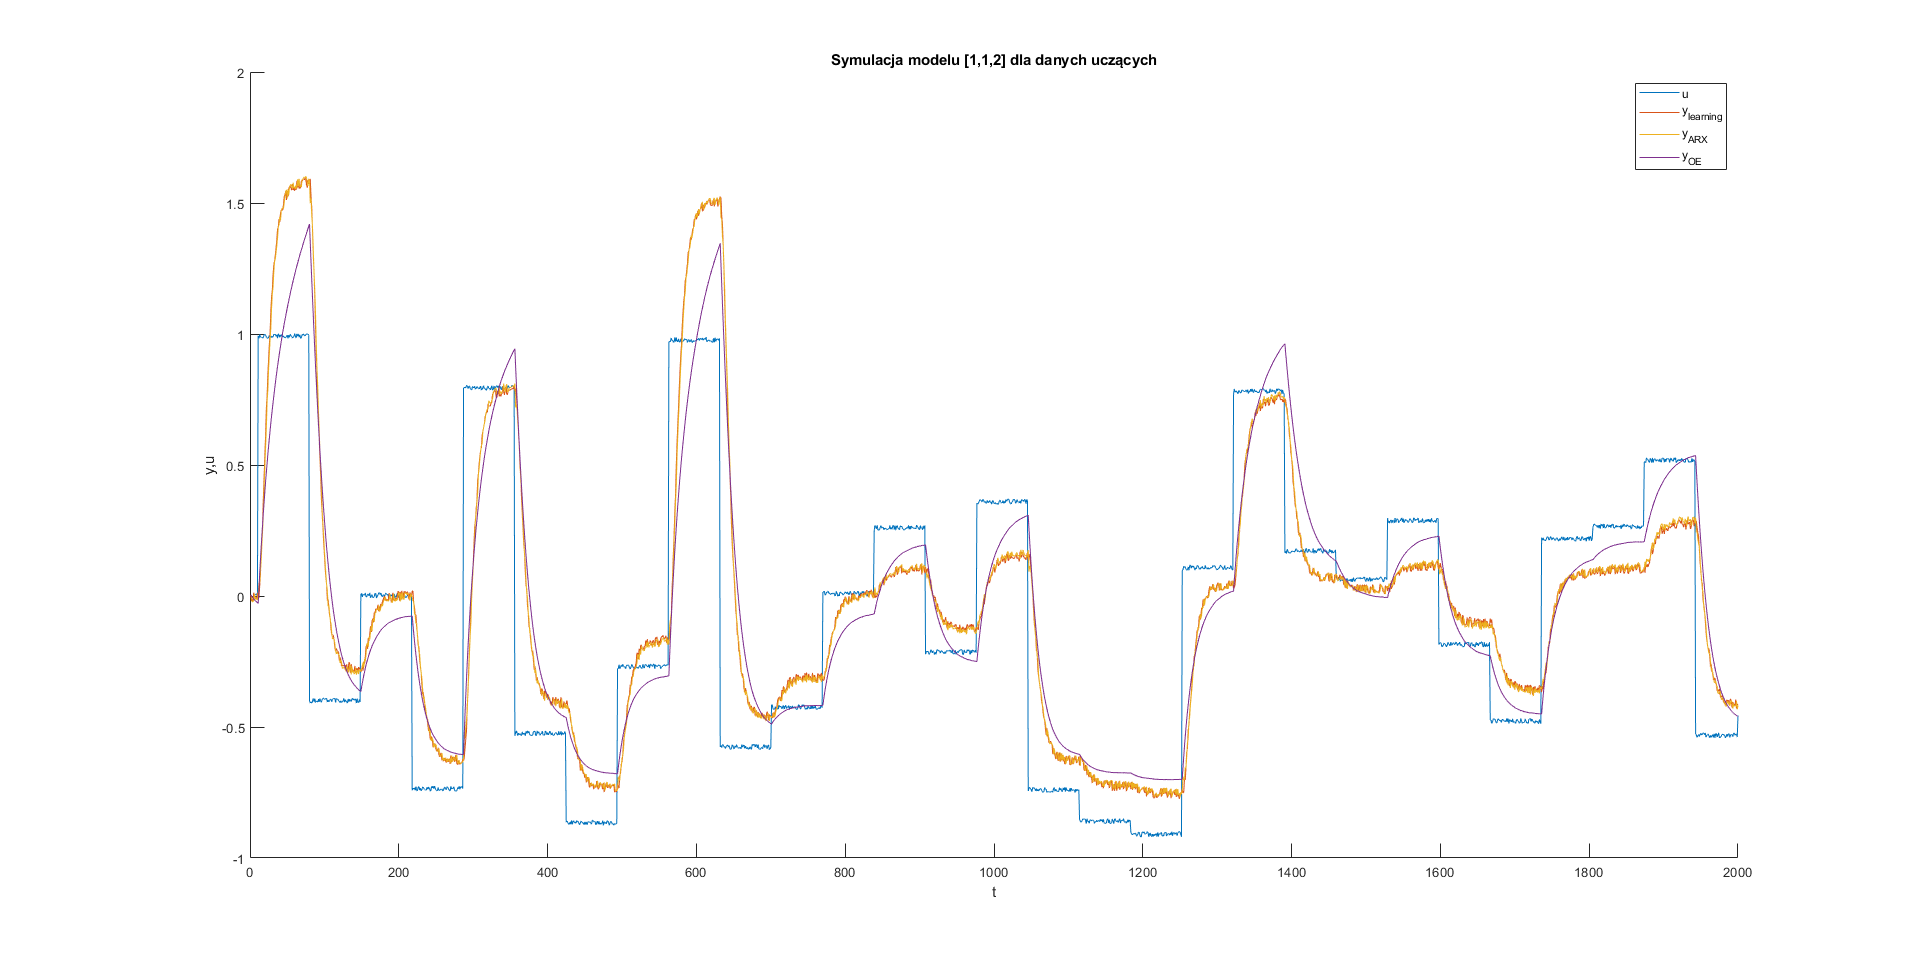
\includegraphics[width=16cm,trim={5cm 1cm 5cm 1cm},clip]{images/d8.png}
\caption{Działanie modelu dynamicznego o 2. stopniu wielomianu i rzędowi dynamiki 1. dla zbioru uczącego.}
\label{fig:d8}
\end{figure}
\begin{figure}[H]
\centering
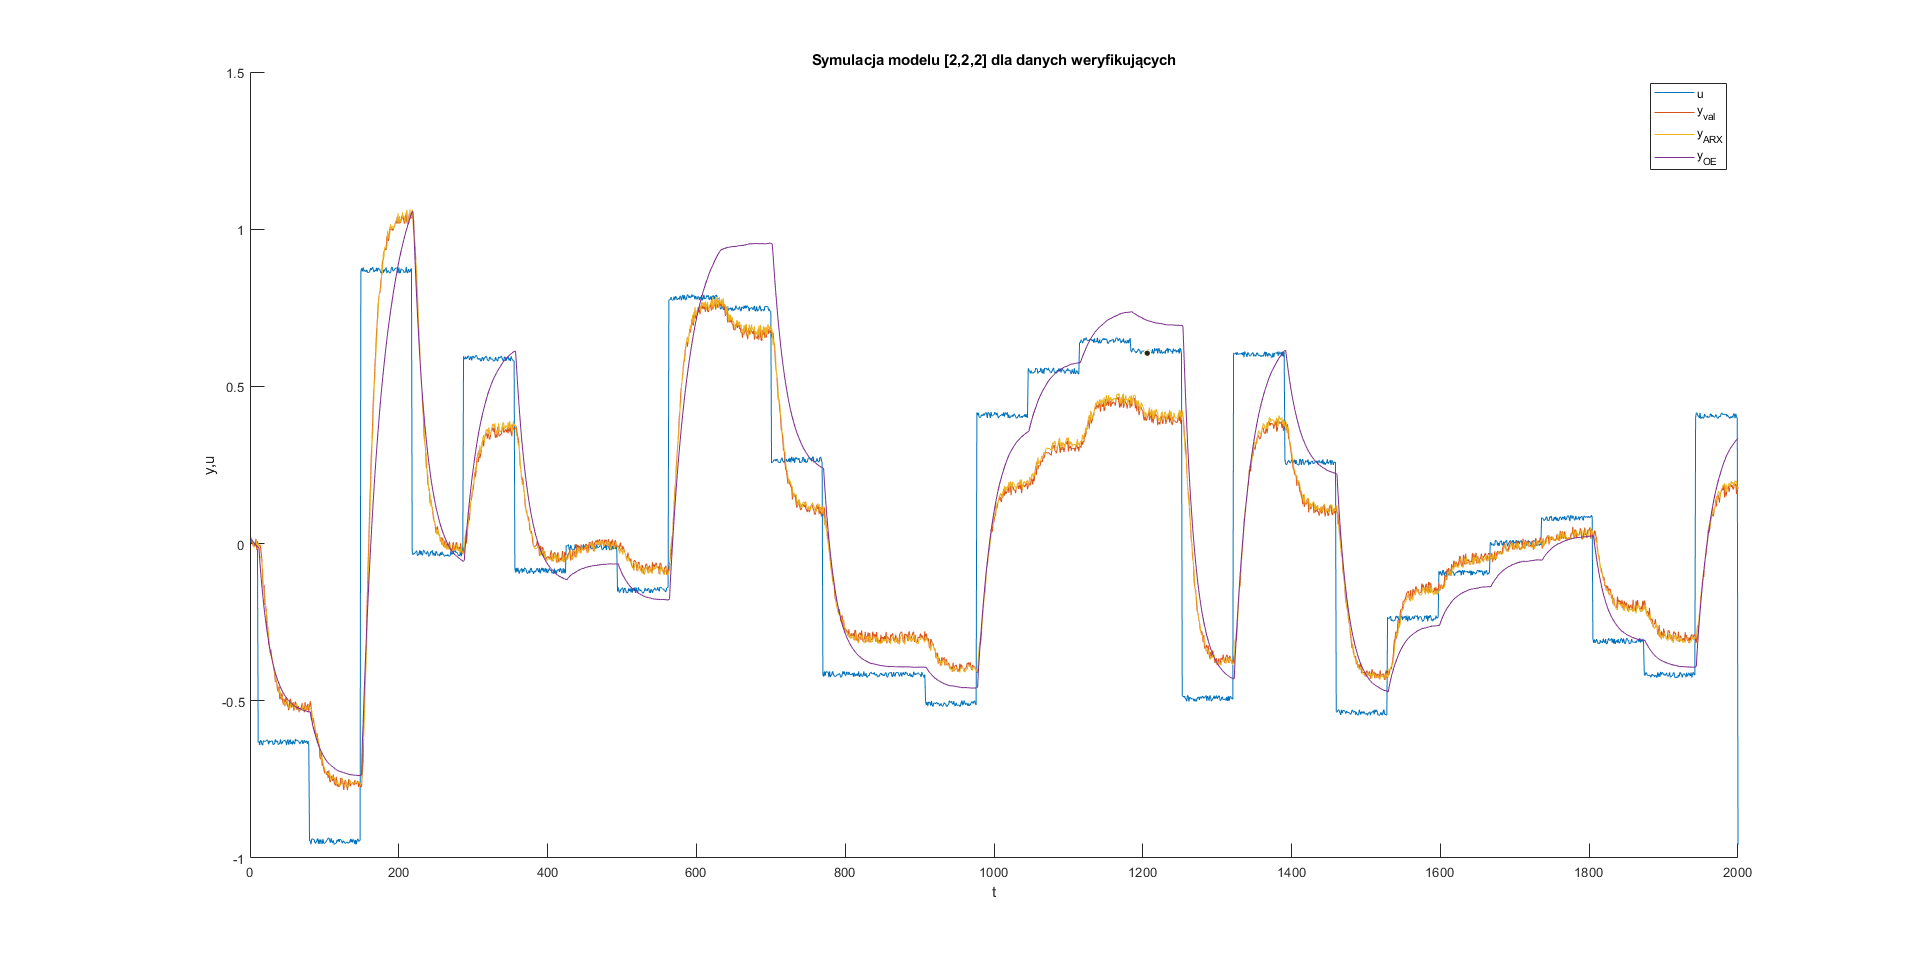
\includegraphics[width=16cm,trim={5cm 1cm 5cm 1cm},clip]{images/d9.png}
\caption{Działanie modelu dynamicznego o 2. stopniu wielomianu i rzędowi dynamiki 2. dla zbioru weryfikującego.}
\label{fig:d9}
\end{figure}
\begin{figure}[H]
\centering
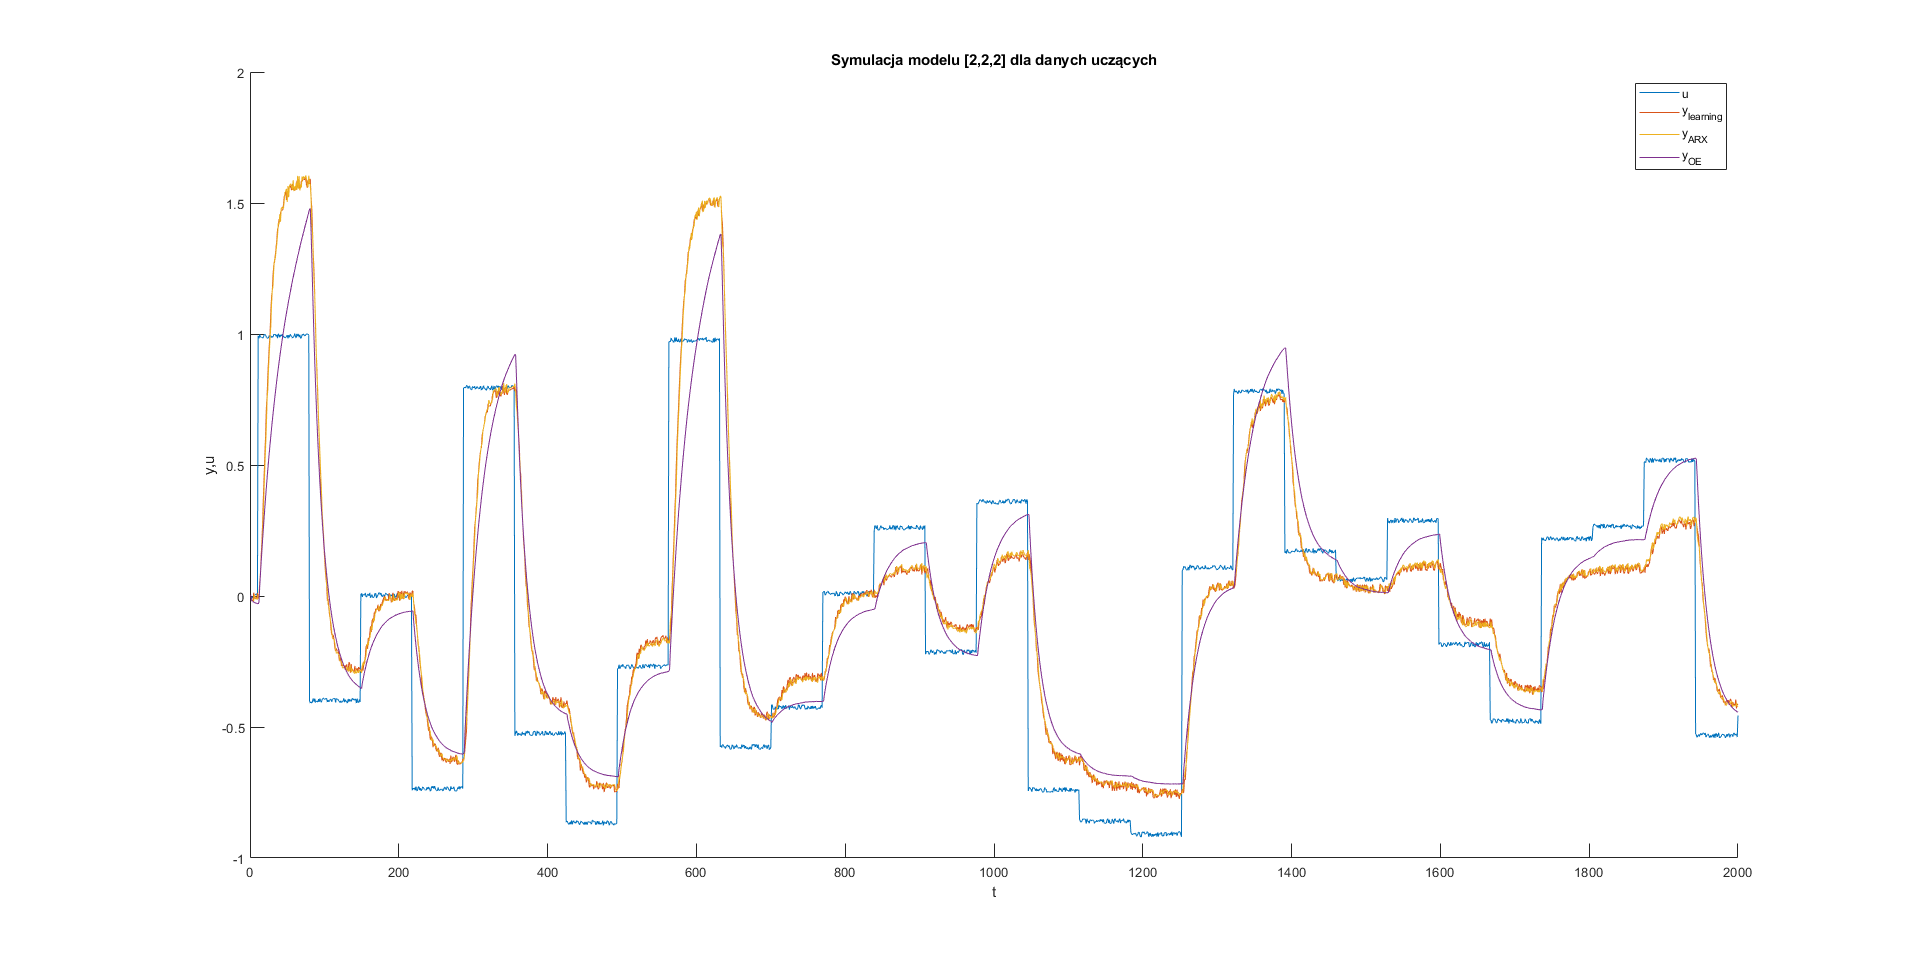
\includegraphics[width=16cm,trim={5cm 1cm 5cm 1cm},clip]{images/d10.png}
\caption{Działanie modelu dynamicznego o 2. stopniu wielomianu i rzędowi dynamiki 2. dla zbioru uczącego.}
\label{fig:d10}
\end{figure}
\begin{figure}[H]
\centering
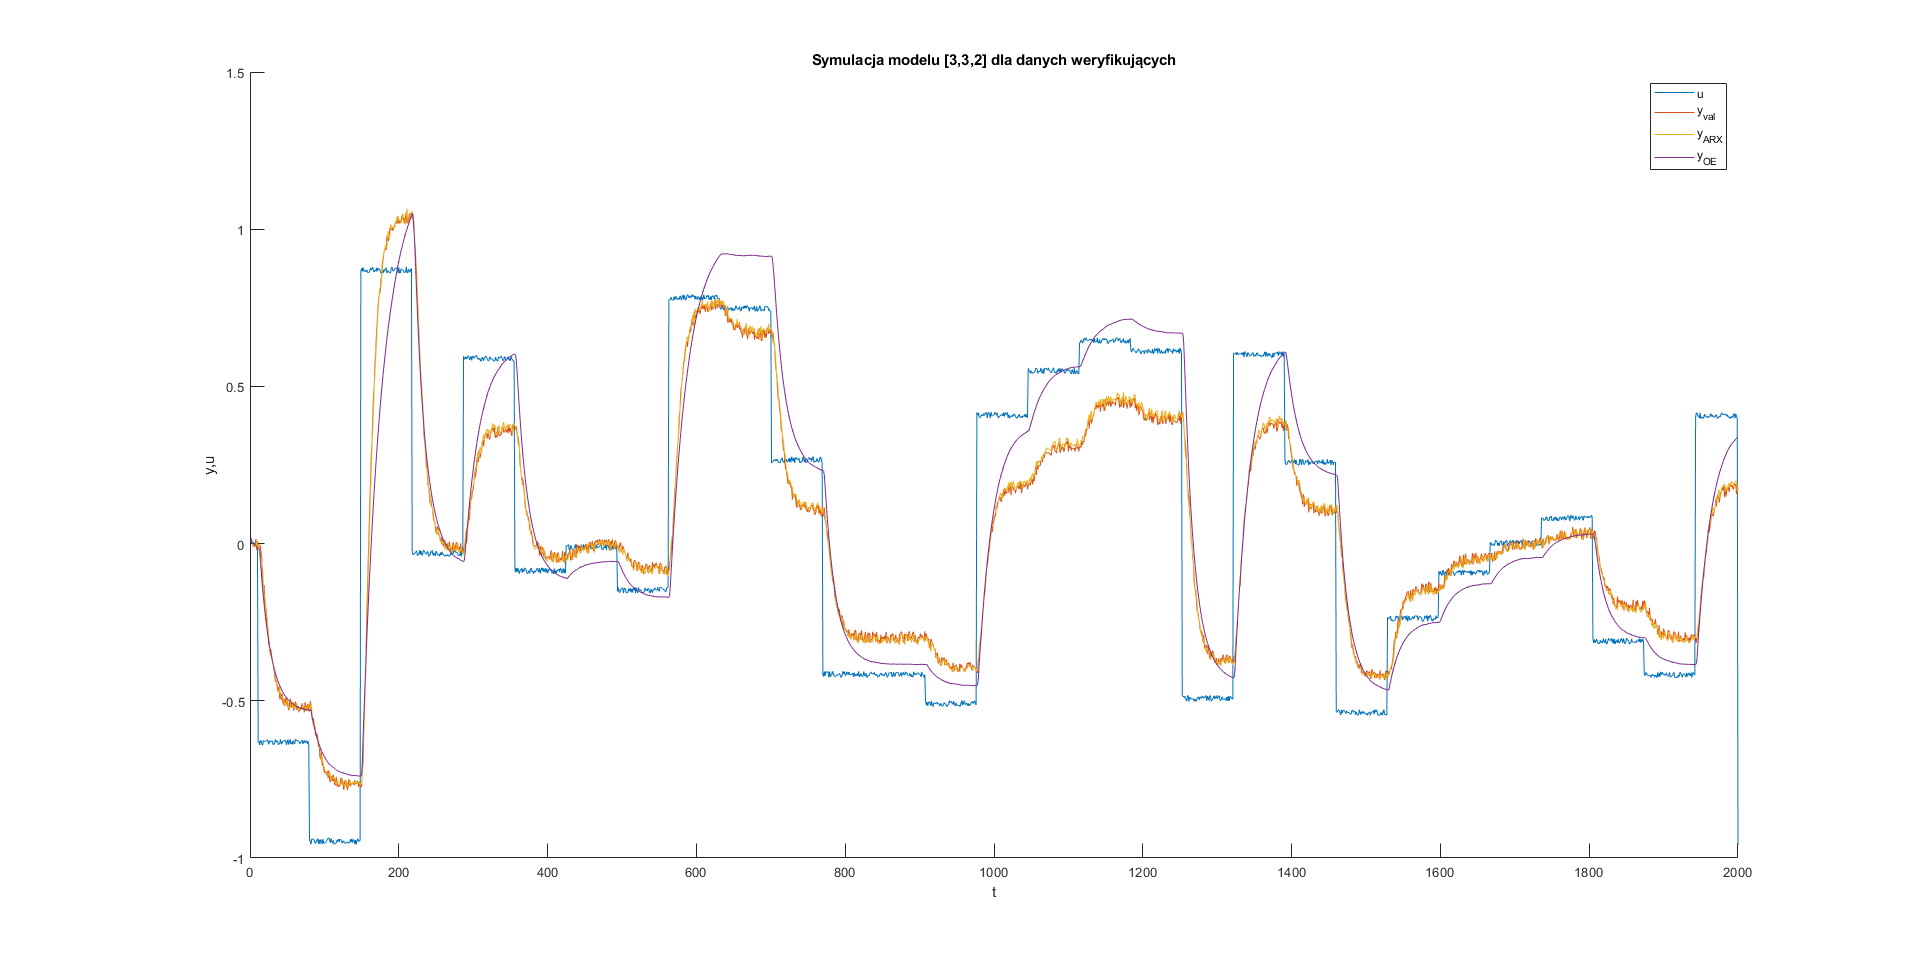
\includegraphics[width=16cm,trim={5cm 1cm 5cm 1cm},clip]{images/d11.png}
\caption{Działanie modelu dynamicznego o 2. stopniu wielomianu i rzędowi dynamiki 3. dla zbioru weryfikującego.}
\label{fig:d11}
\end{figure}
\begin{figure}[H]
\centering
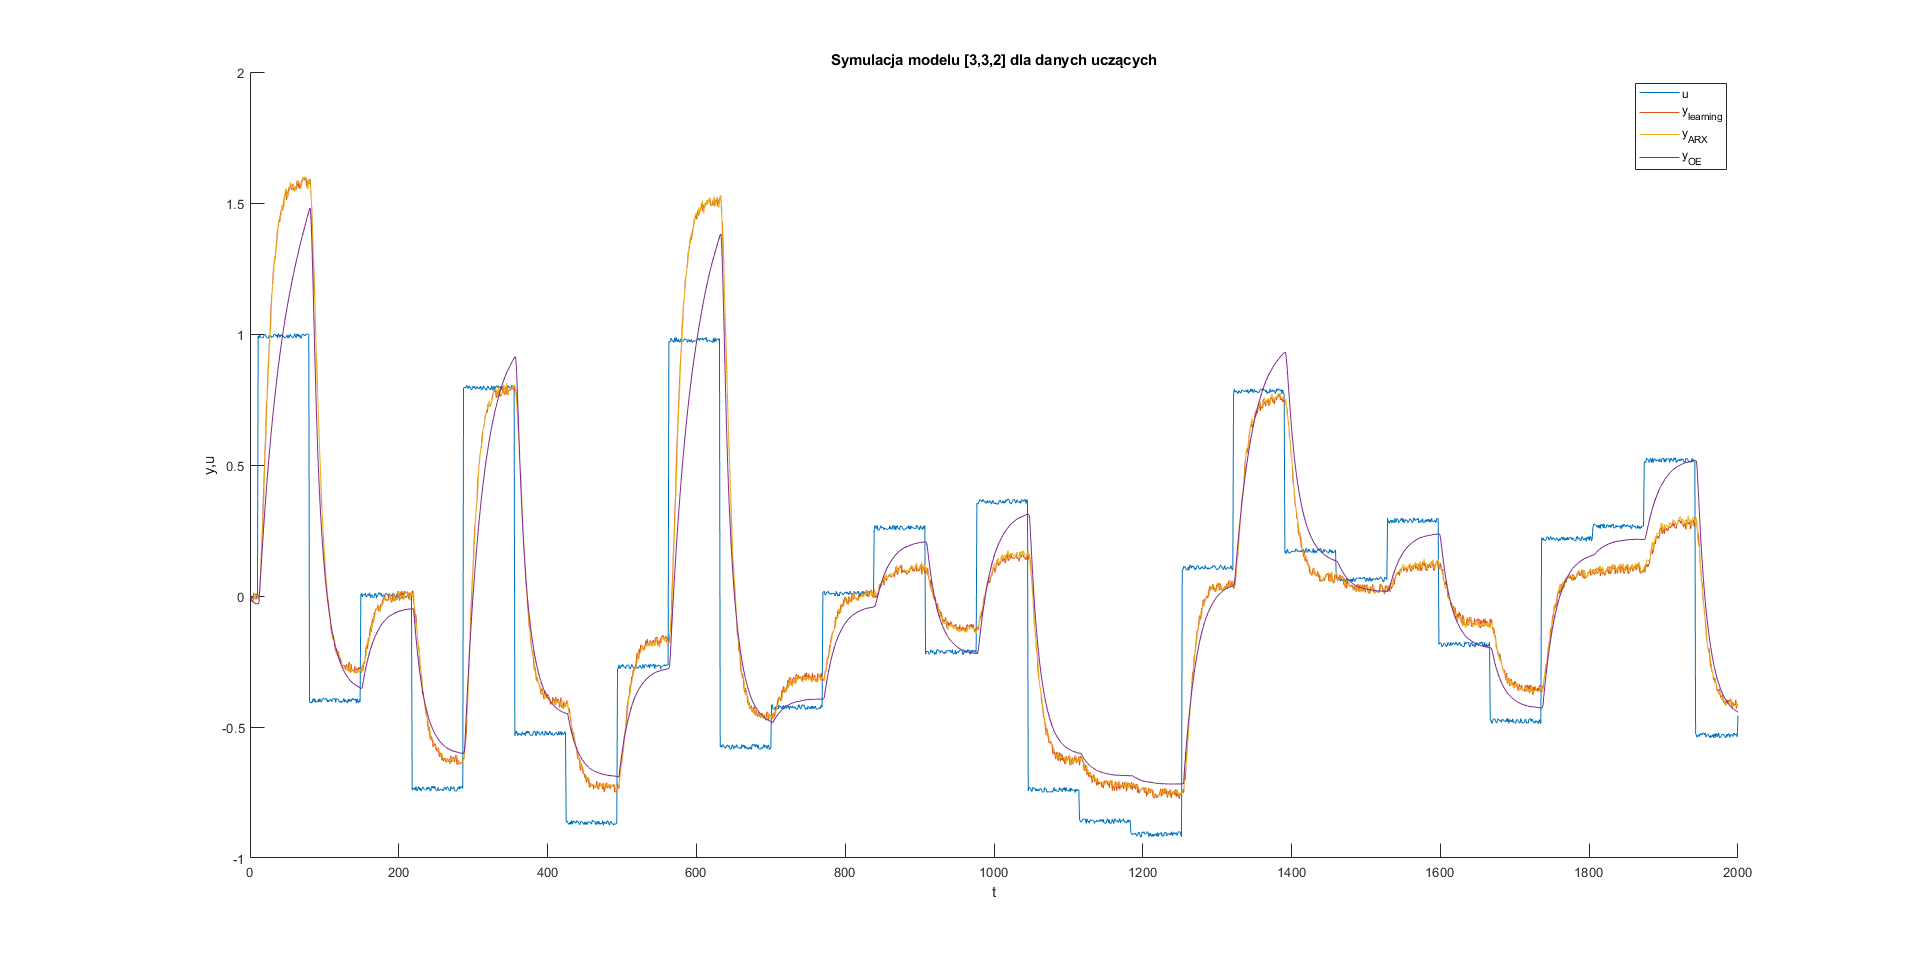
\includegraphics[width=16cm,trim={5cm 1cm 5cm 1cm},clip]{images/d12.png}
\caption{Działanie modelu dynamicznego o 2. stopniu wielomianu i rzędowi dynamiki 3. dla zbioru uczącego.}
\label{fig:d12}
\end{figure}
\subsubsection{Modele z wielomianem 3. stopnia}
\begin{figure}[H]
\centering
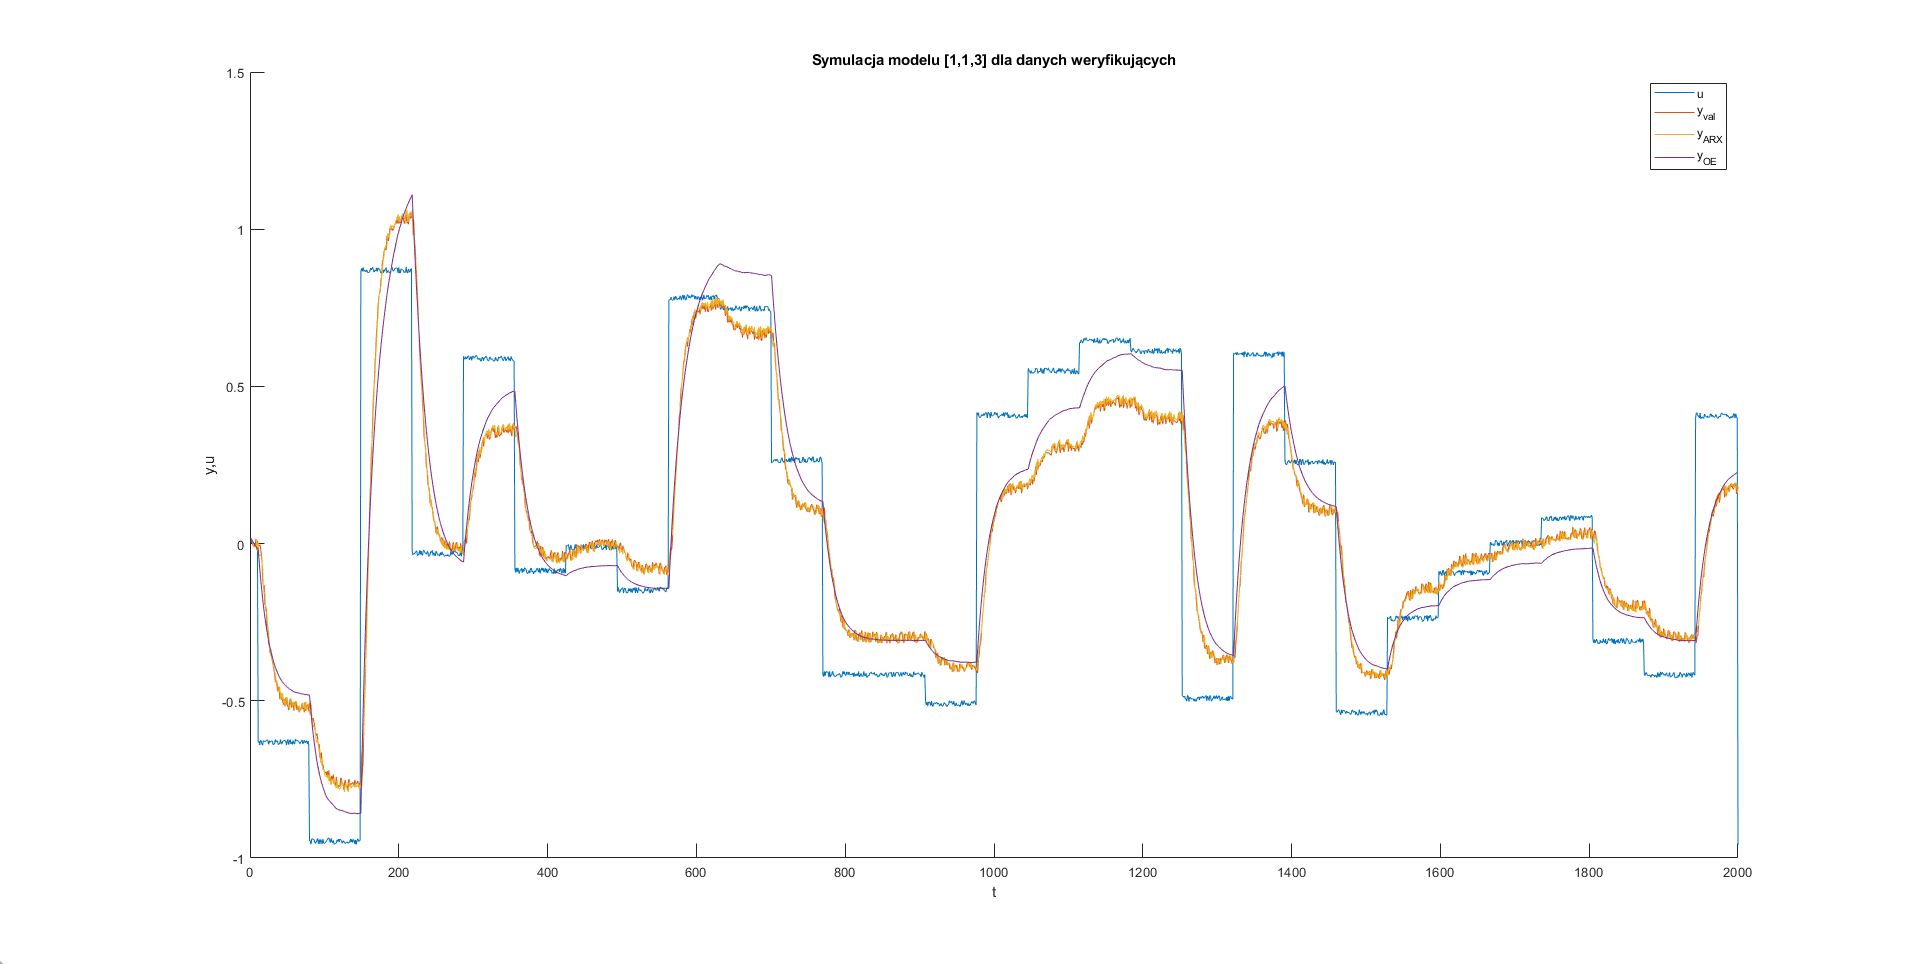
\includegraphics[width=16cm,trim={5cm 1cm 5cm 1cm},clip]{images/d13.png}
\caption{Działanie modelu dynamicznego o 3. stopniu wielomianu i rzędowi dynamiki 1. dla zbioru weryfikującego.}
\label{fig:d13}
\end{figure}
\begin{figure}[H]
\centering
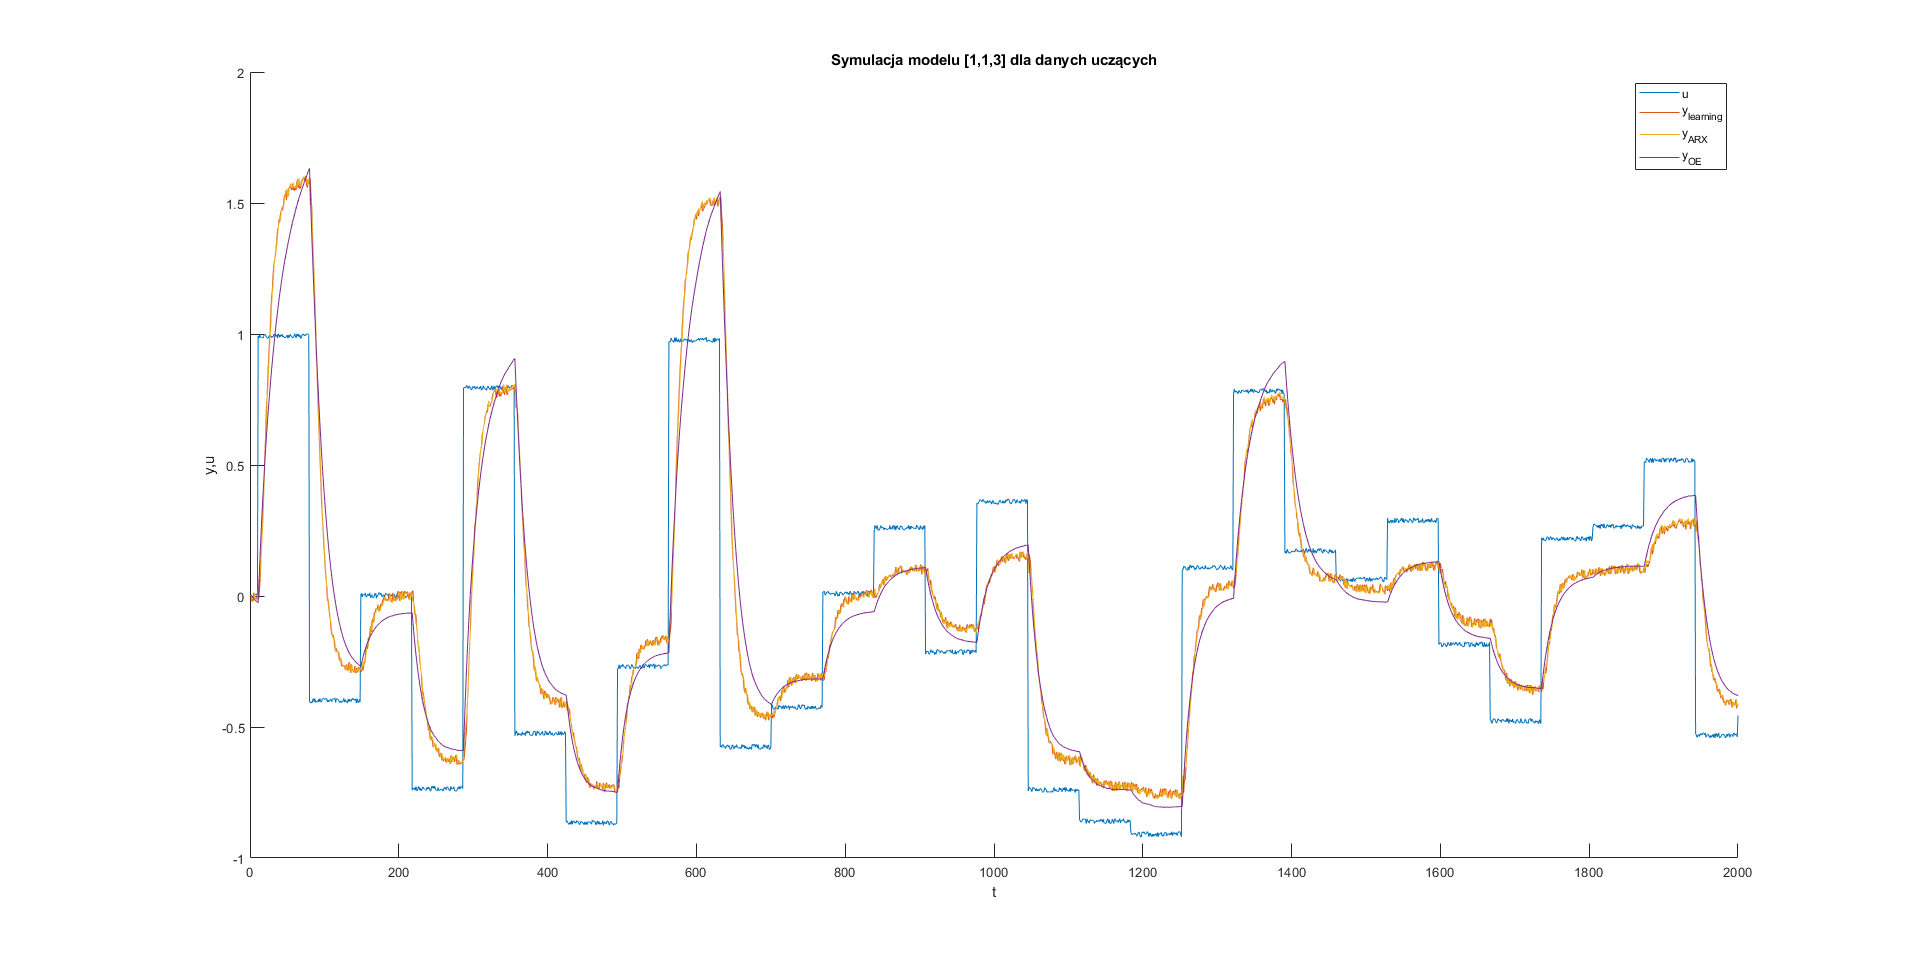
\includegraphics[width=16cm,trim={5cm 1cm 5cm 1cm},clip]{images/d14.png}
\caption{Działanie modelu dynamicznego o 3. stopniu wielomianu i rzędowi dynamiki 1. dla zbioru uczącego.}
\label{fig:d14}
\end{figure}
\begin{figure}[H]
\centering
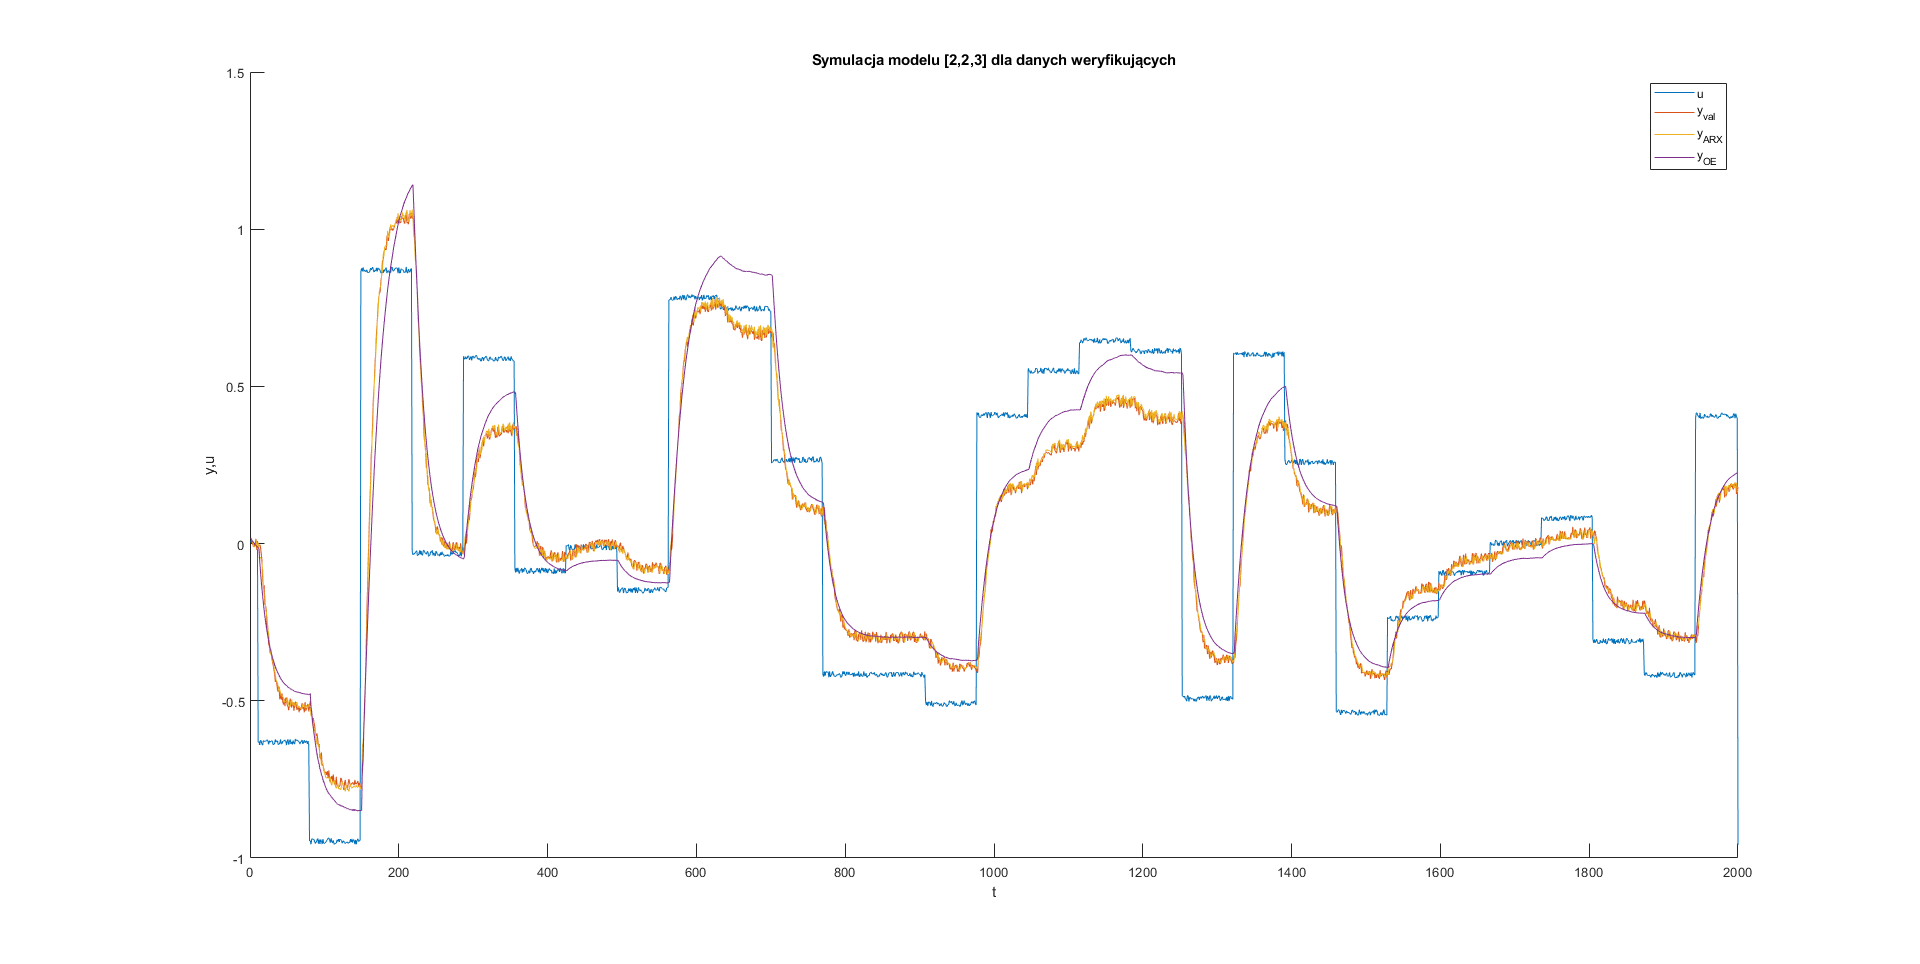
\includegraphics[width=16cm,trim={5cm 1cm 5cm 1cm},clip]{images/d15.png}
\caption{Działanie modelu dynamicznego o 3. stopniu wielomianu i rzędowi dynamiki 2. dla zbioru weryfikującego.}
\label{fig:d15}
\end{figure}
\begin{figure}[H]
\centering
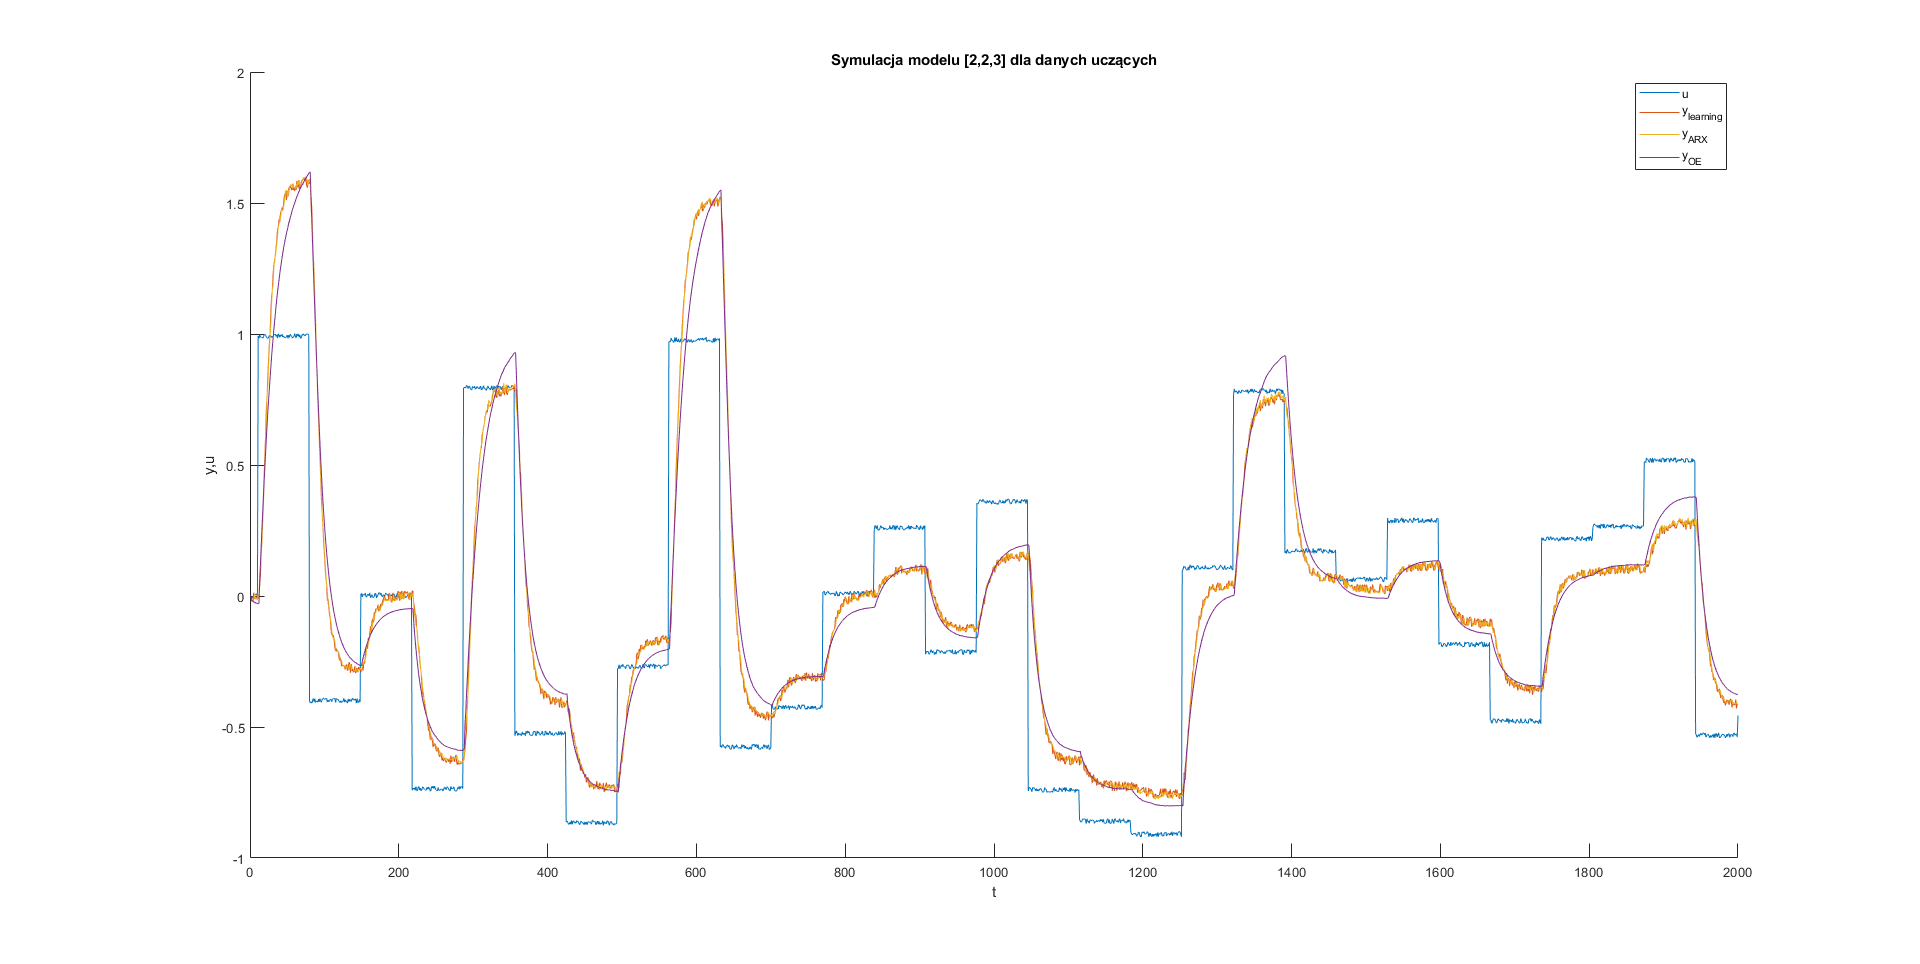
\includegraphics[width=16cm,trim={5cm 1cm 5cm 1cm},clip]{images/d16.png}
\caption{Działanie modelu dynamicznego o 3. stopniu wielomianu i rzędowi dynamiki 2. dla zbioru uczącego.}
\label{fig:d16}
\end{figure}
\begin{figure}[H]
\centering
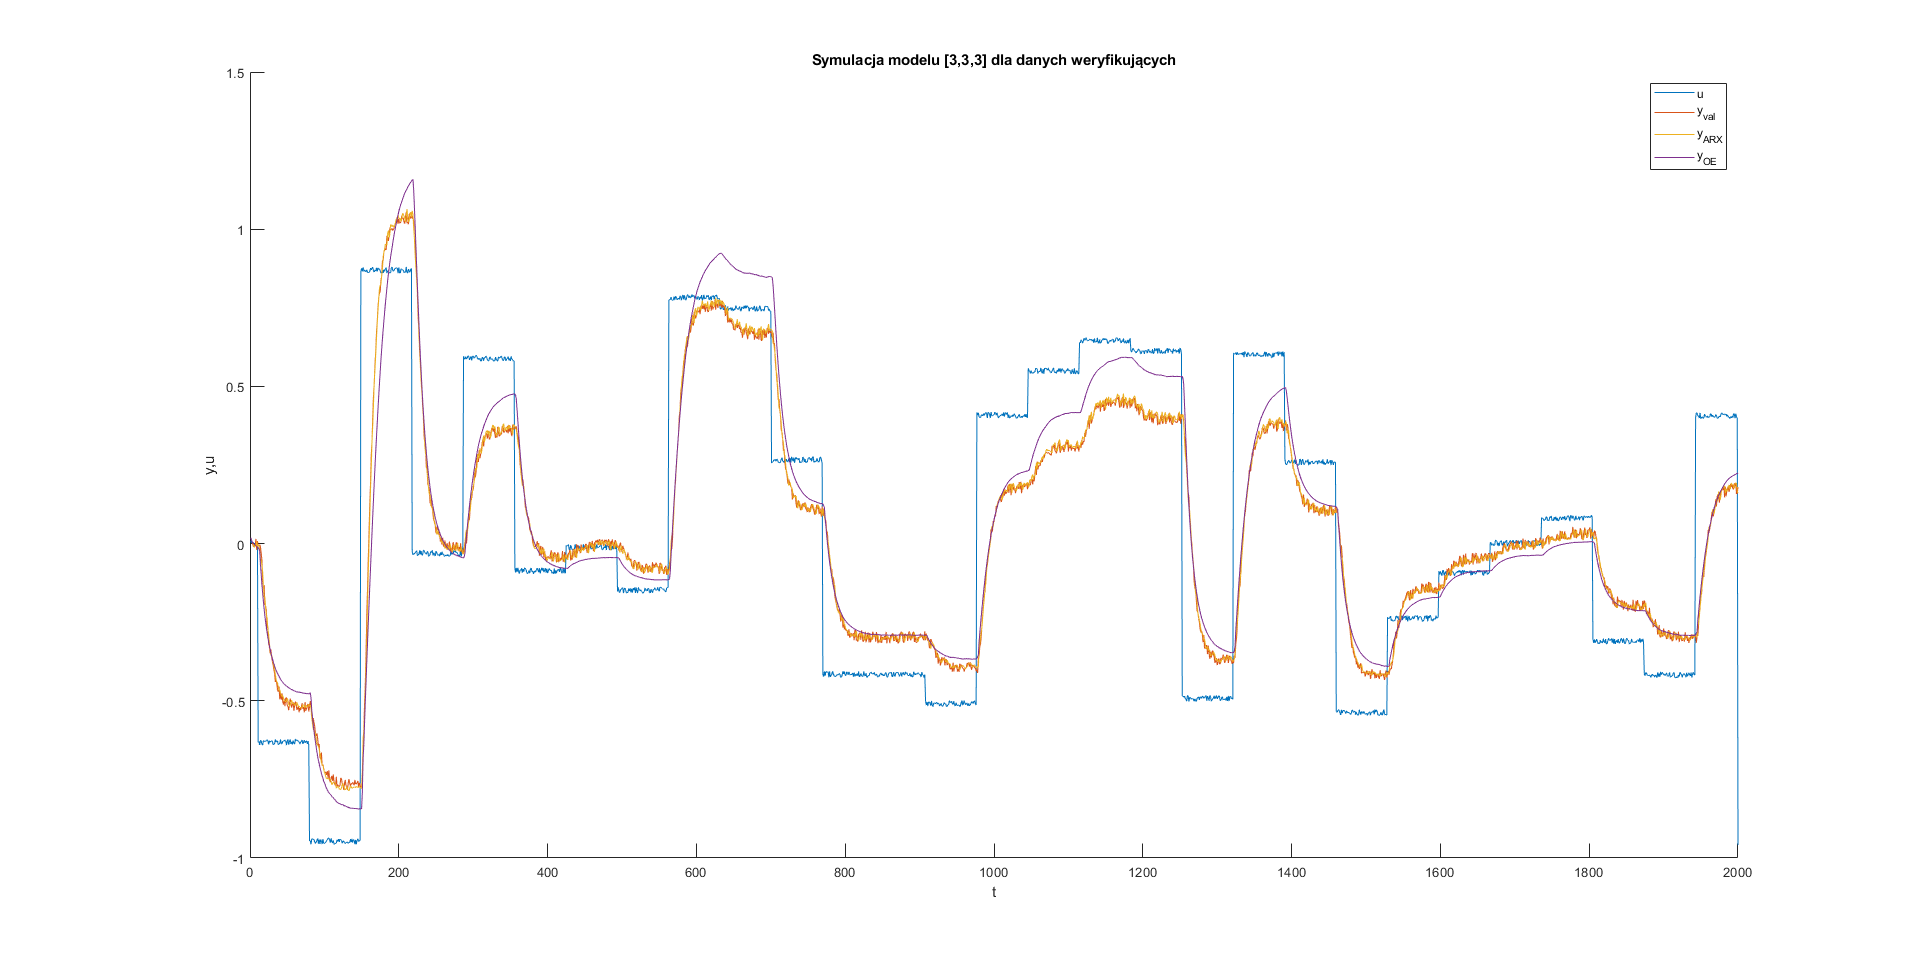
\includegraphics[width=16cm,trim={5cm 1cm 5cm 1cm},clip]{images/d17.png}
\caption{Działanie modelu dynamicznego o 3. stopniu wielomianu i rzędowi dynamiki 3. dla zbioru weryfikującego.}
\label{fig:d17}
\end{figure}
\begin{figure}[H]
\centering
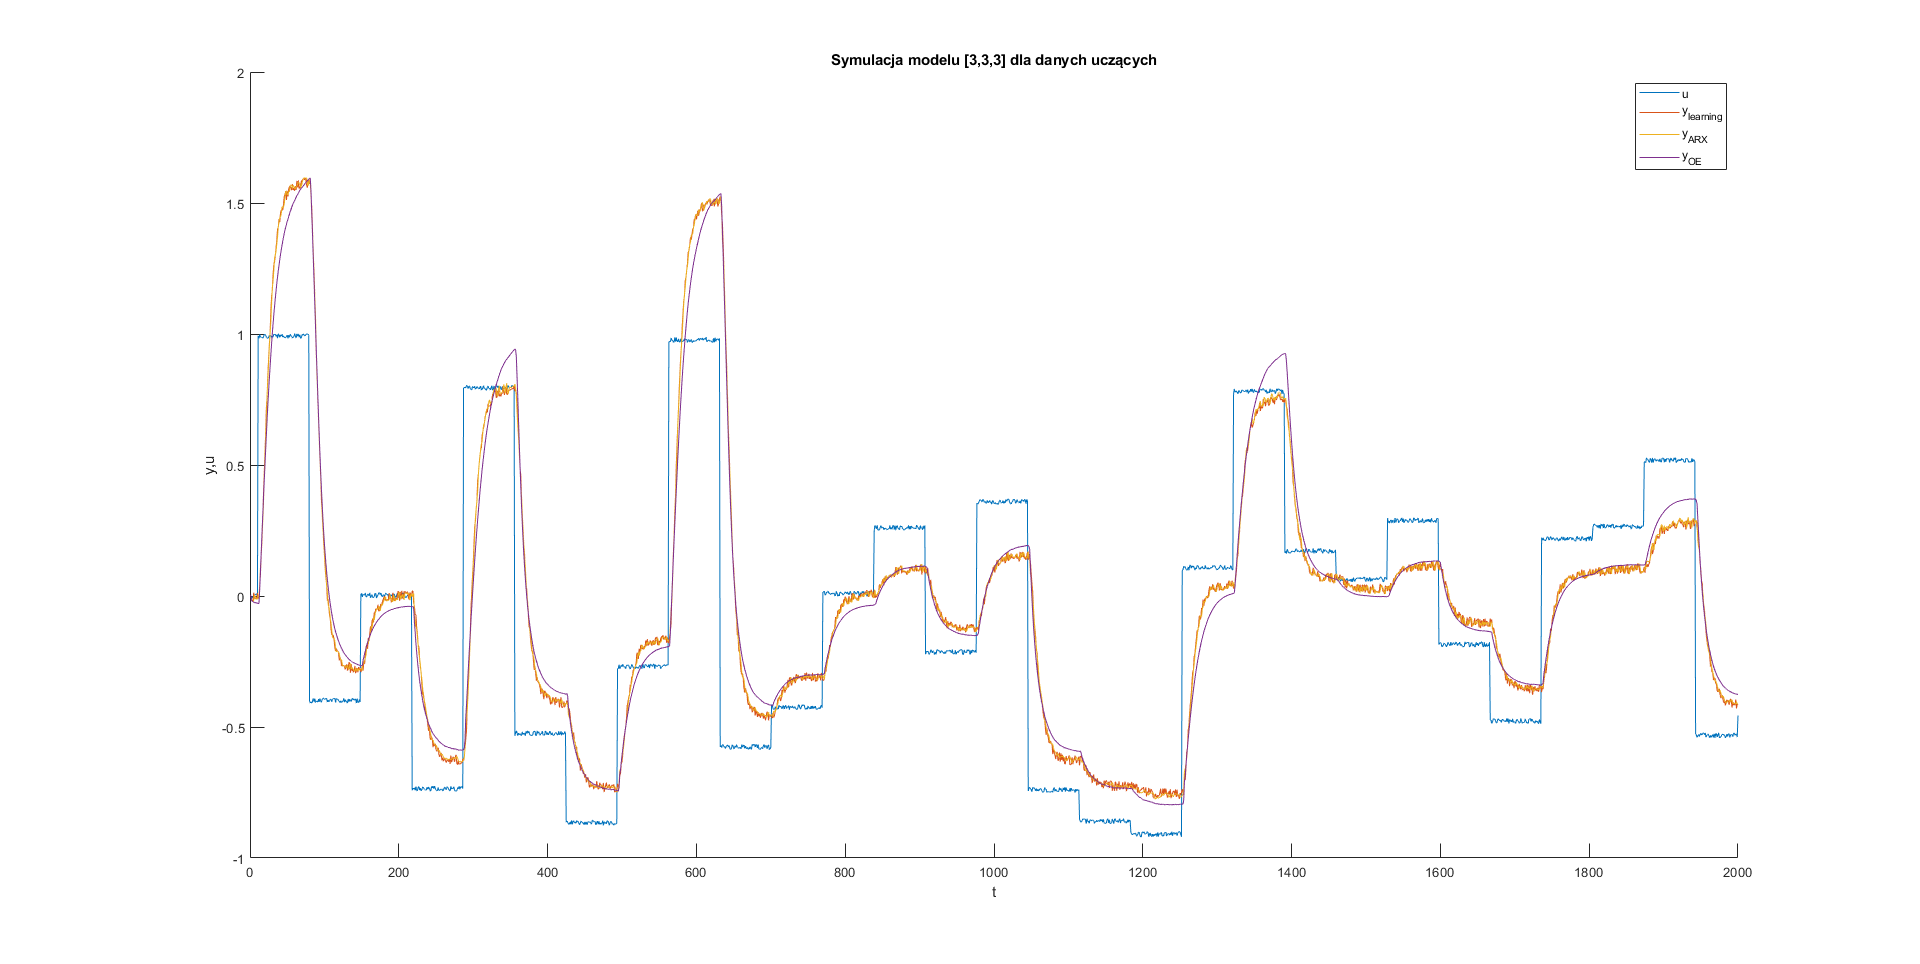
\includegraphics[width=16cm,trim={5cm 1cm 5cm 1cm},clip]{images/d18.png}
\caption{Działanie modelu dynamicznego o 3. stopniu wielomianu i rzędowi dynamiki 3. dla zbioru uczącego.}
\label{fig:d18}
\end{figure}
\subsubsection{Modele z wielomianem 4. stopnia}
\begin{figure}[H]
\centering
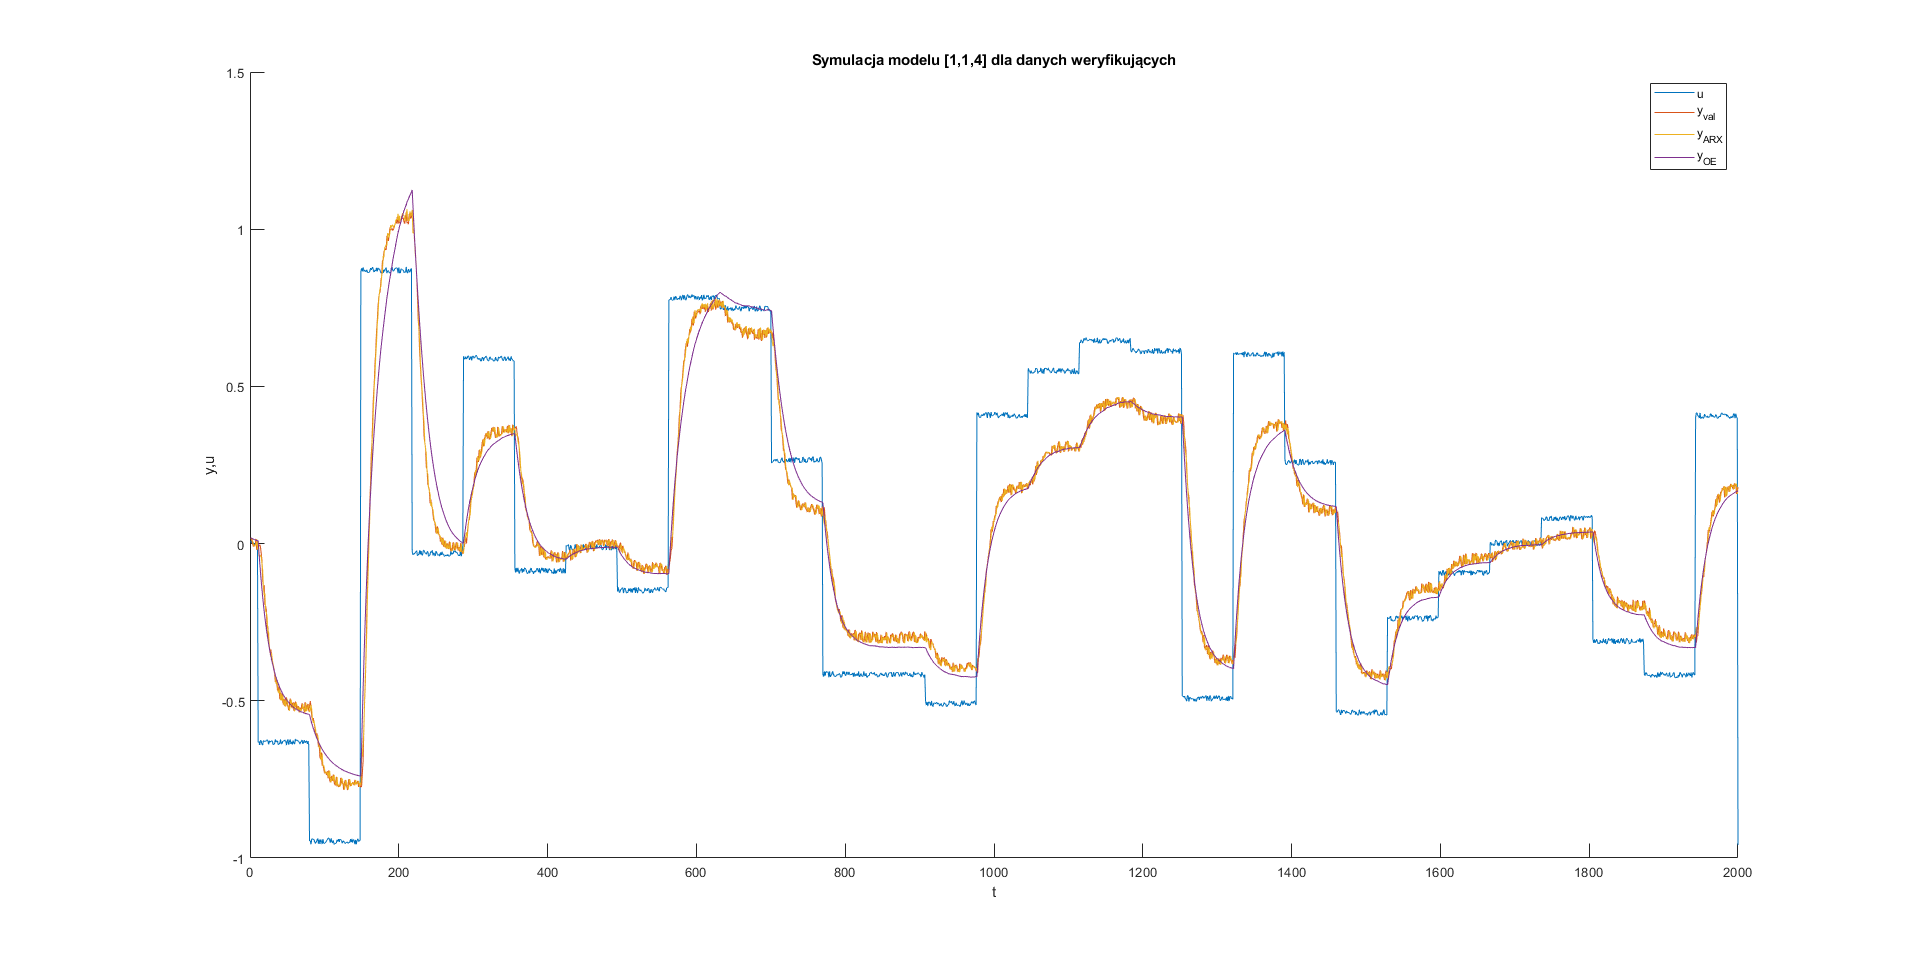
\includegraphics[width=16cm,trim={5cm 1cm 5cm 1cm},clip]{images/d19.png}
\caption{Działanie modelu dynamicznego o 4. stopniu wielomianu i rzędowi dynamiki 1. dla zbioru weryfikującego.}
\label{fig:d19}
\end{figure}
\begin{figure}[H]
\centering
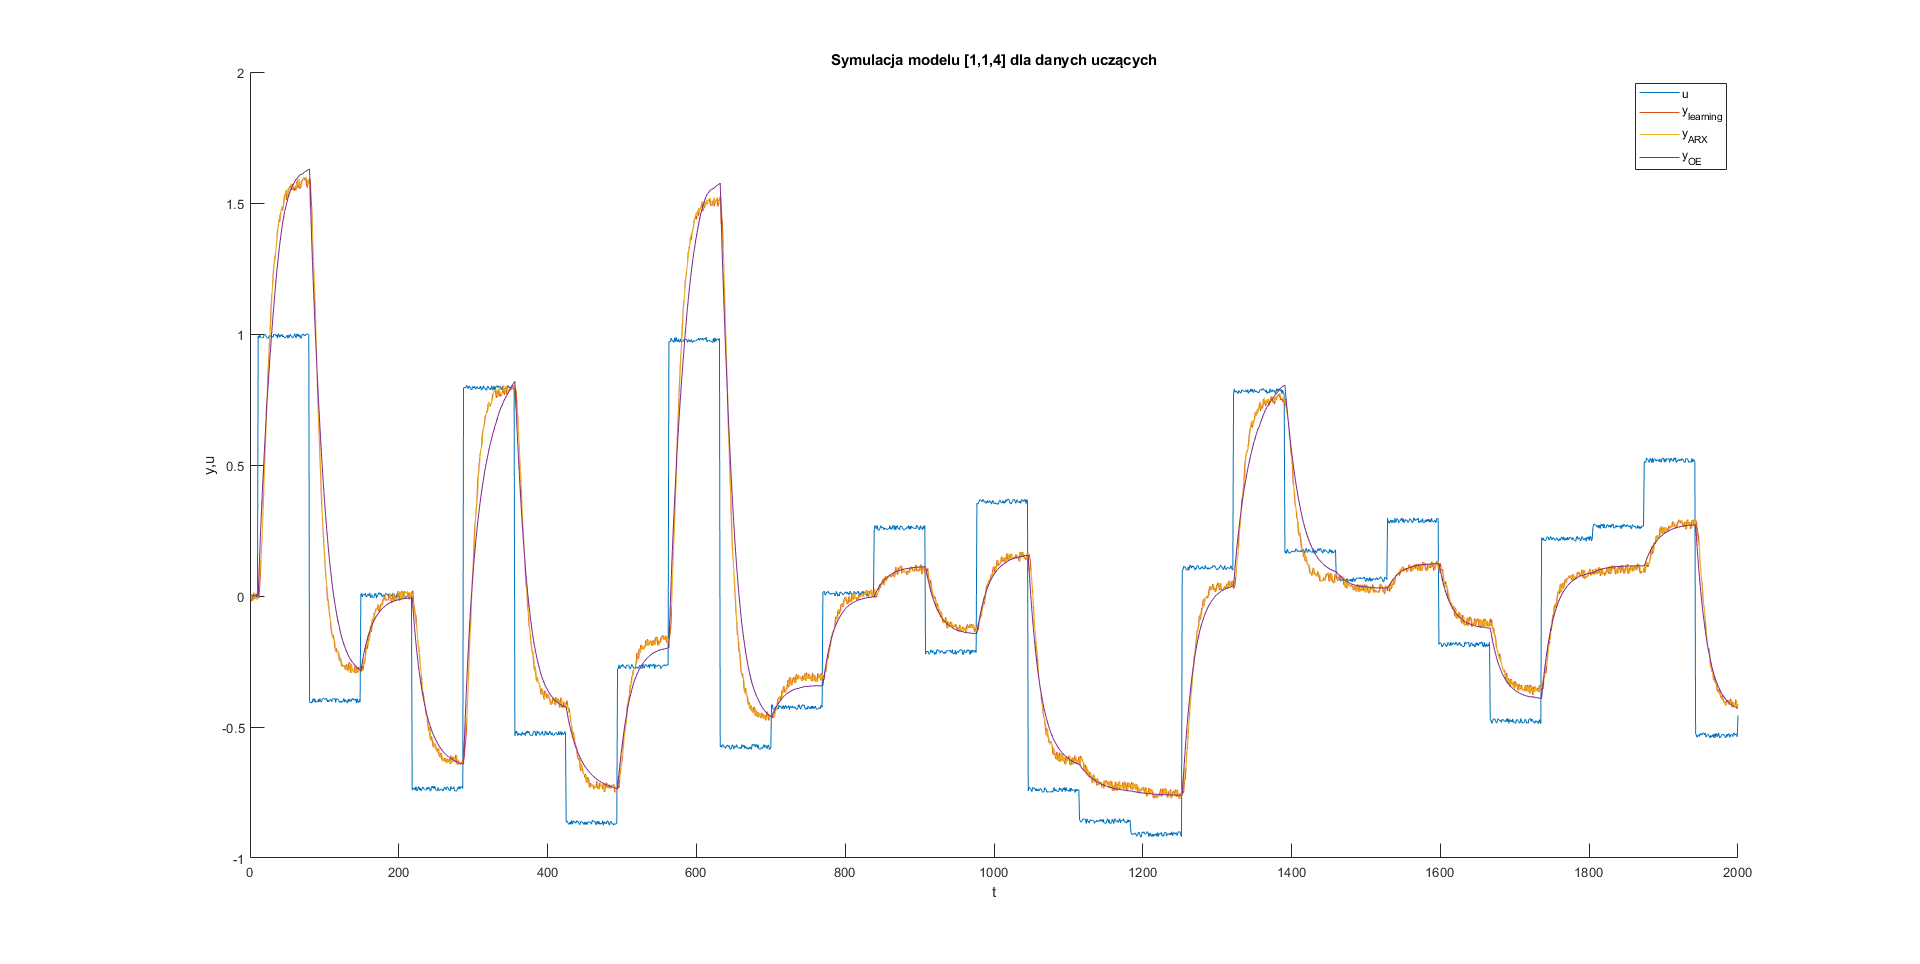
\includegraphics[width=16cm,trim={5cm 1cm 5cm 1cm},clip]{images/d20.png}
\caption{Działanie modelu dynamicznego o 4. stopniu wielomianu i rzędowi dynamiki 1. dla zbioru uczącego.}
\label{fig:d20}
\end{figure}
\begin{figure}[H]
\centering
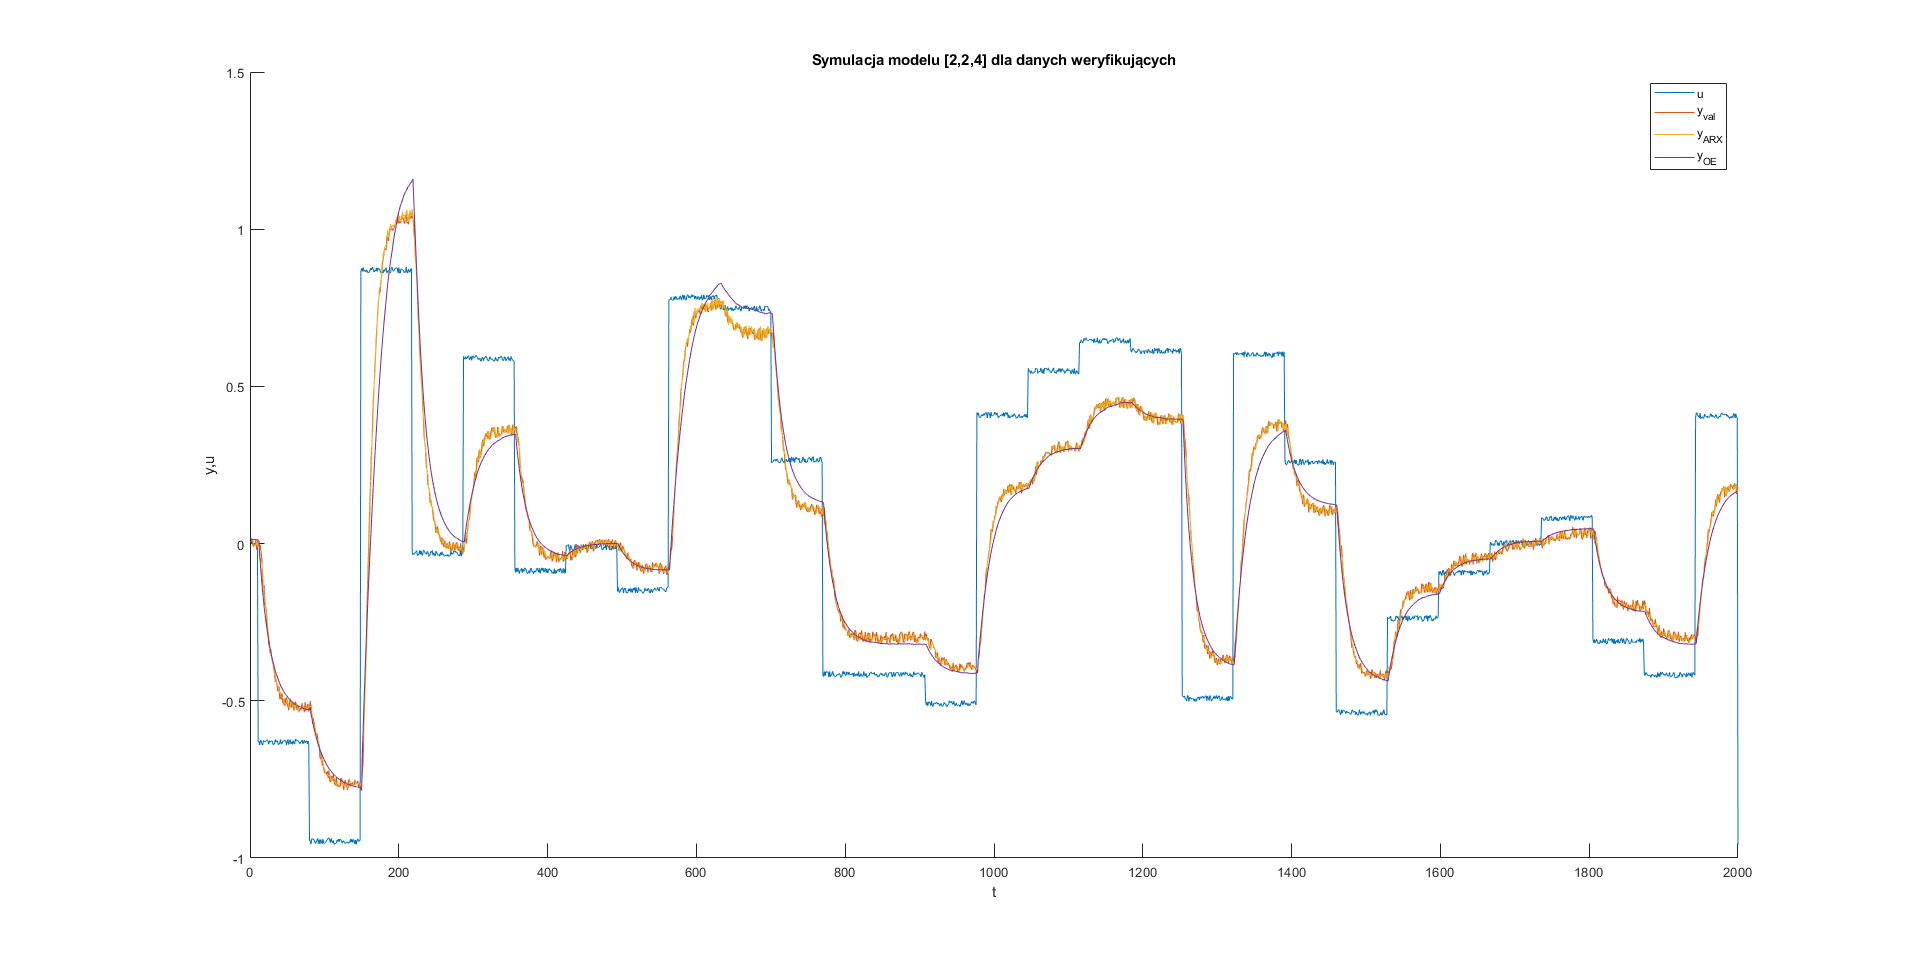
\includegraphics[width=16cm,trim={5cm 1cm 5cm 1cm},clip]{images/d21.png}
\caption{Działanie modelu dynamicznego o 4. stopniu wielomianu i rzędowi dynamiki 2. dla zbioru weryfikującego.}
\label{fig:d21}
\end{figure}
\begin{figure}[H]
\centering
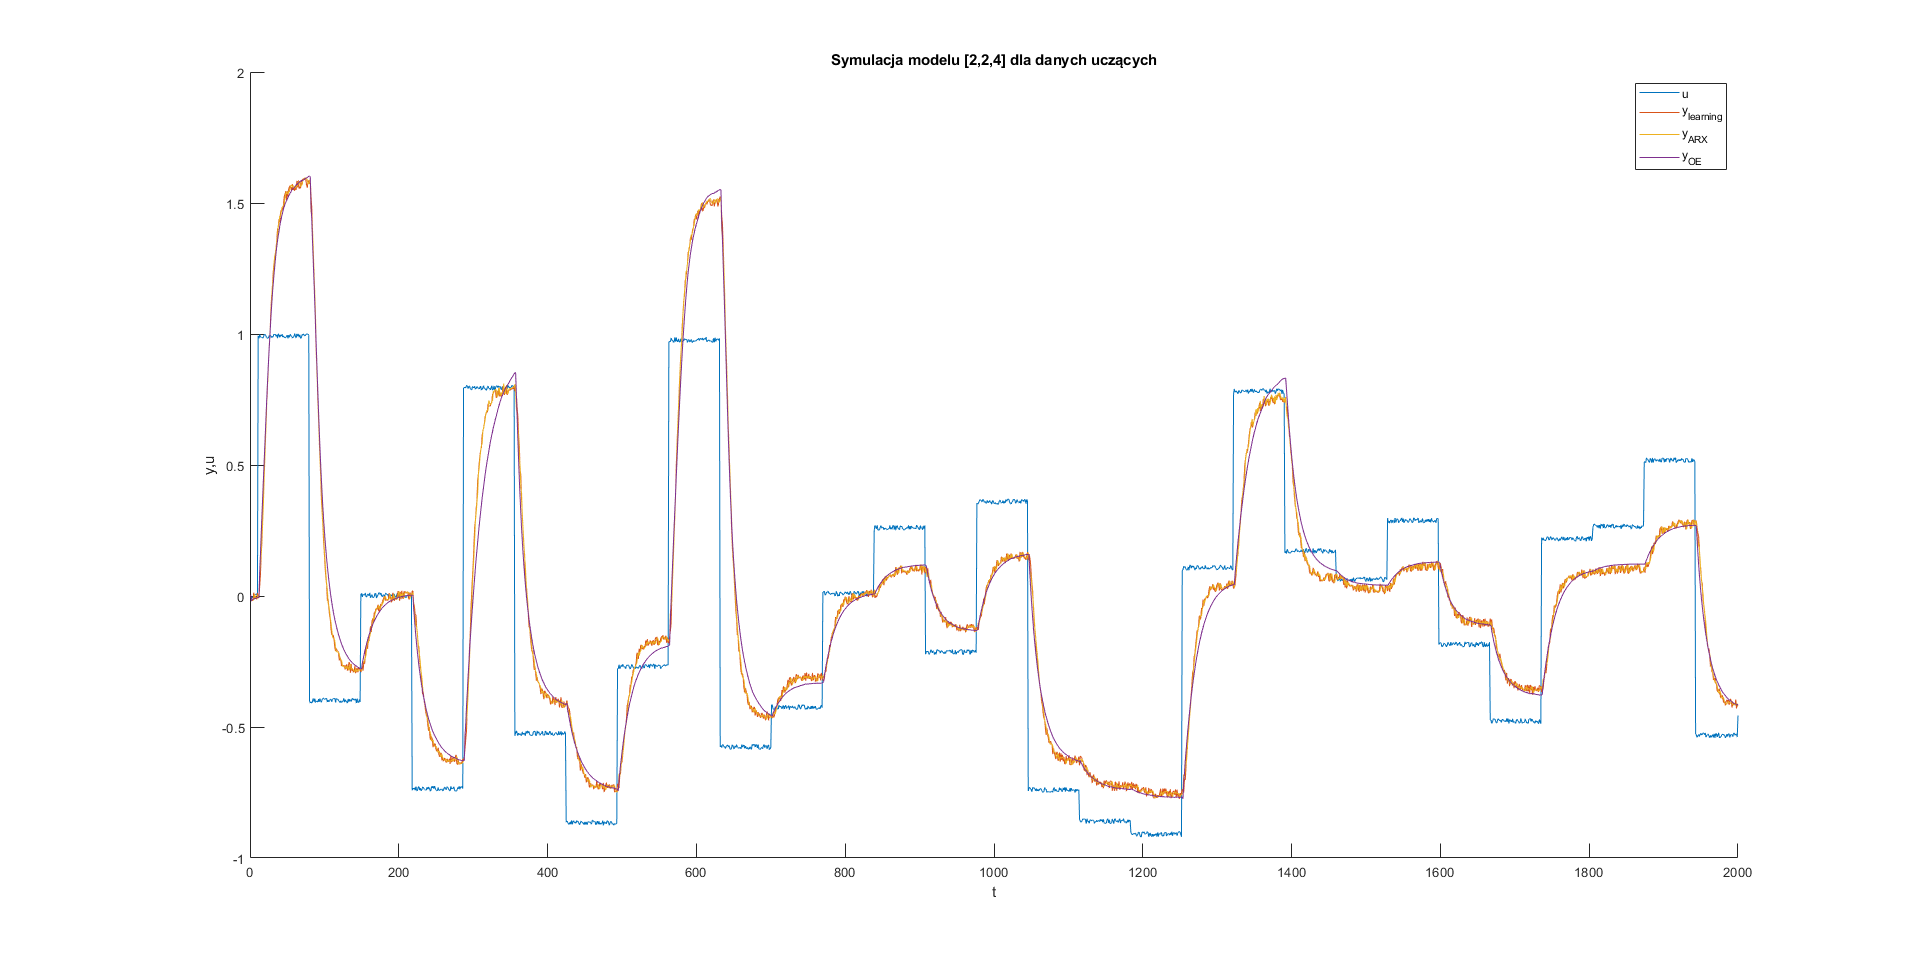
\includegraphics[width=16cm,trim={5cm 1cm 5cm 1cm},clip]{images/d22.png}
\caption{Działanie modelu dynamicznego o 4. stopniu wielomianu i rzędowi dynamiki 2. dla zbioru uczącego.}
\label{fig:d22}
\end{figure}
\begin{figure}[H]
\centering
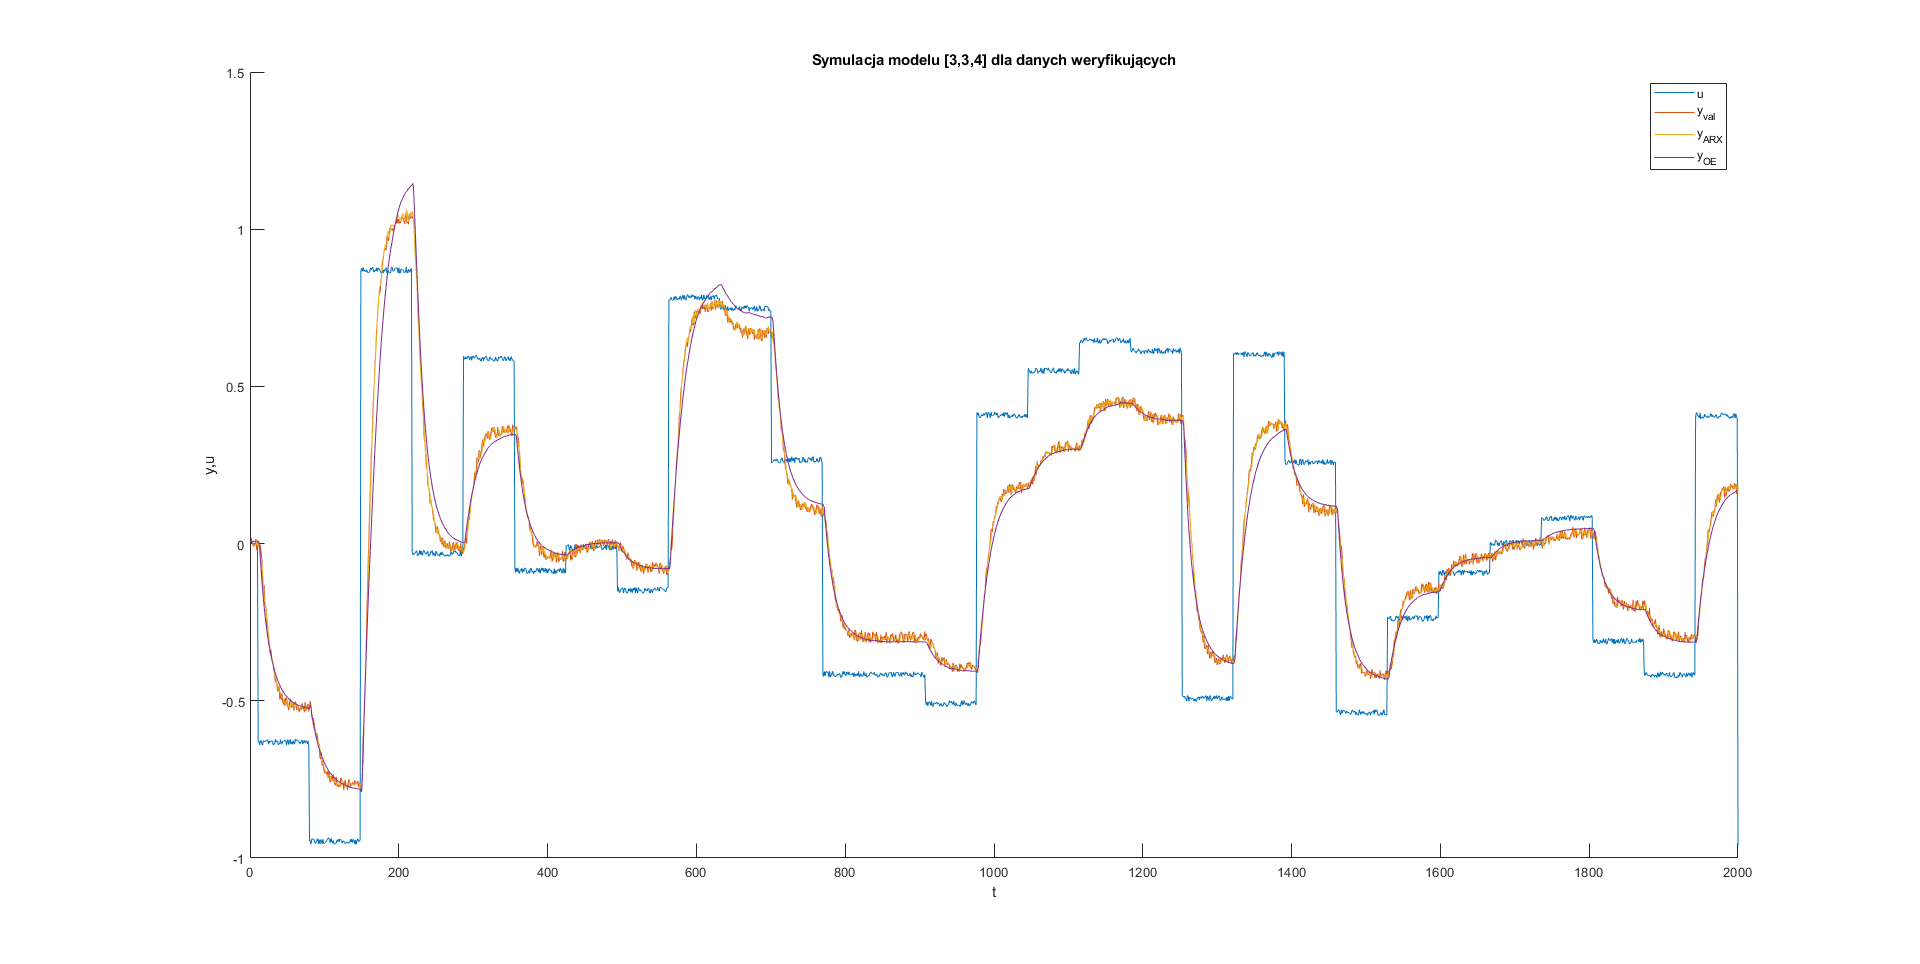
\includegraphics[width=16cm,trim={5cm 1cm 5cm 1cm},clip]{images/d23.png}
\caption{Działanie modelu dynamicznego o 4. stopniu wielomianu i rzędowi dynamiki 3. dla zbioru weryfikującego.}
\label{fig:d23}
\end{figure}
\begin{figure}[H]
\centering
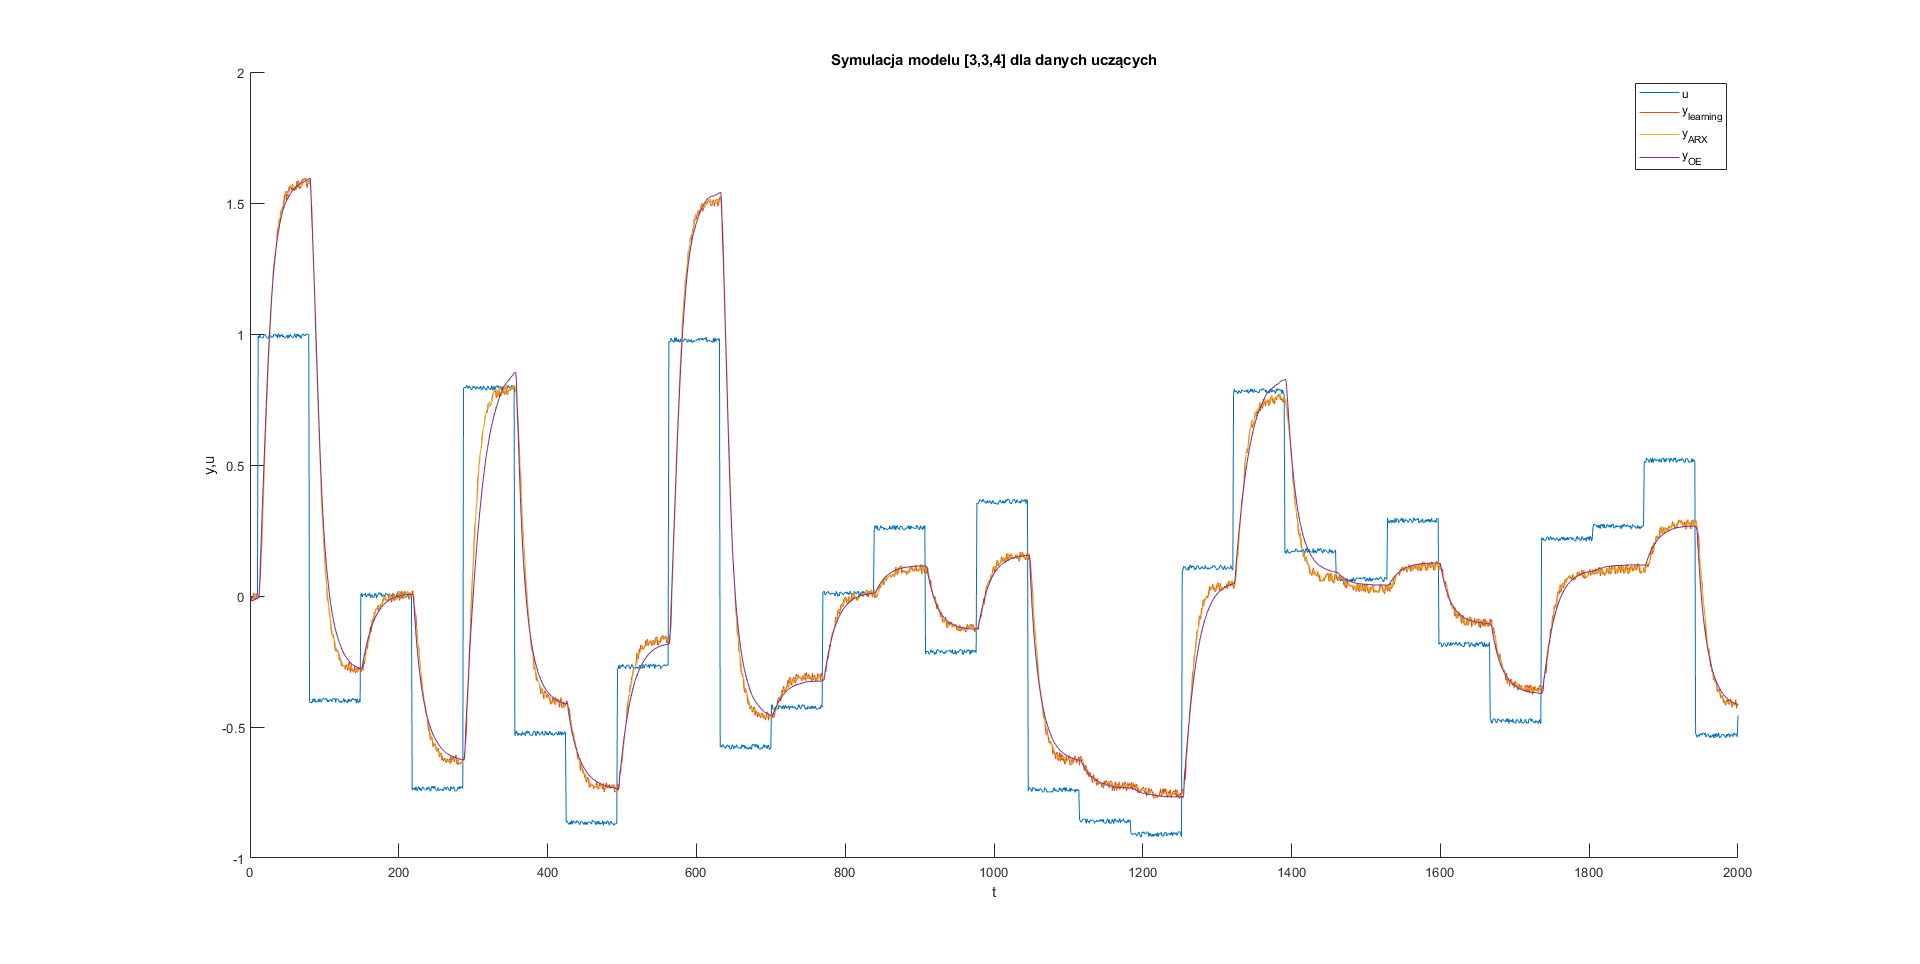
\includegraphics[width=16cm,trim={5cm 1cm 5cm 1cm},clip]{images/d24.png}
\caption{Działanie modelu dynamicznego o 4. stopniu wielomianu i rzędowi dynamiki 3. dla zbioru uczącego.}
\label{fig:d24}
\end{figure}
\subsubsection{Modele z wielomianem 5. stopnia}
\begin{figure}[H]
\centering
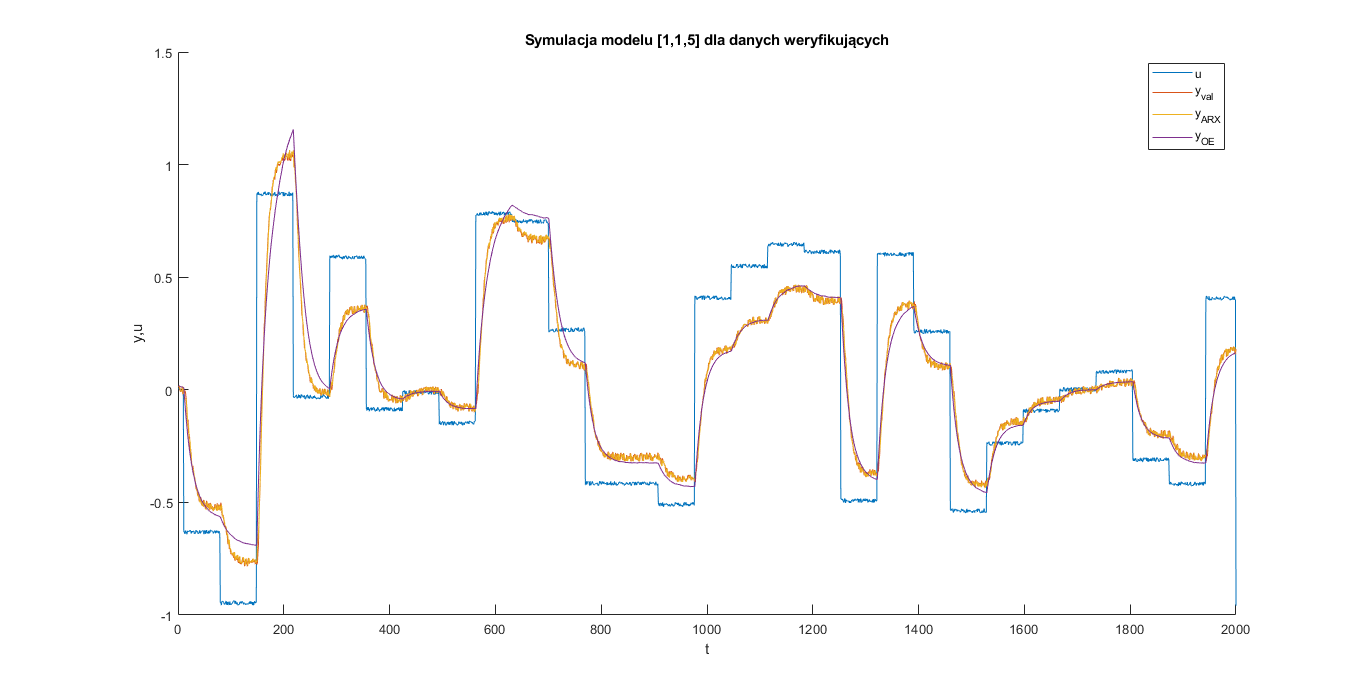
\includegraphics[width=16cm,trim={3cm 0.5cm 3cm 0.5cm},clip]{images/d25.png}
\caption{Działanie modelu dynamicznego o 5. stopniu wielomianu i rzędowi dynamiki 1. dla zbioru weryfikującego.}
\label{fig:d25}
\end{figure}
\begin{figure}[H]
\centering
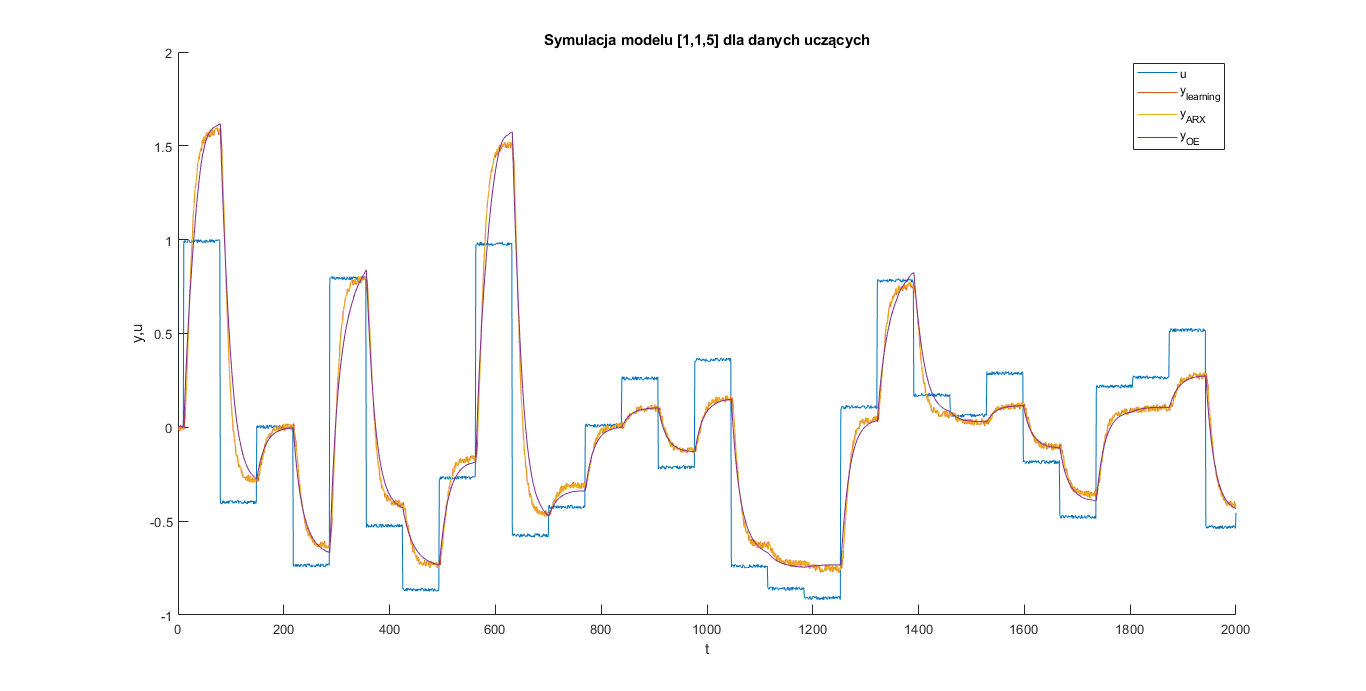
\includegraphics[width=16cm,trim={3cm 0.5cm 3cm 0.5cm},clip]{images/d26.png}
\caption{Działanie modelu dynamicznego o 5. stopniu wielomianu i rzędowi dynamiki 1. dla zbioru uczącego.}
\label{fig:d26}
\end{figure}
\begin{figure}[H]
\centering
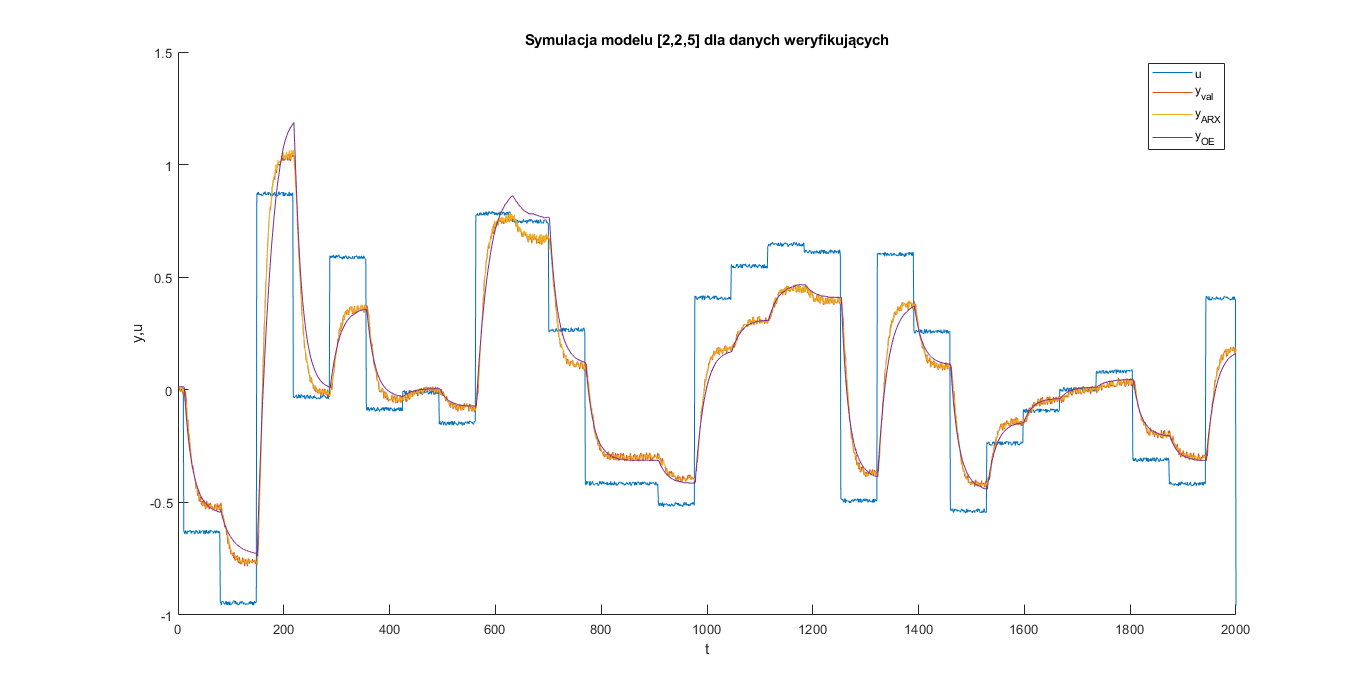
\includegraphics[width=16cm,trim={3cm 0.5cm 3cm 0.5cm},clip]{images/d27.png}
\caption{Działanie modelu dynamicznego o 5. stopniu wielomianu i rzędowi dynamiki 2. dla zbioru weryfikującego.}
\label{fig:d27}
\end{figure}
\begin{figure}[H]
\centering
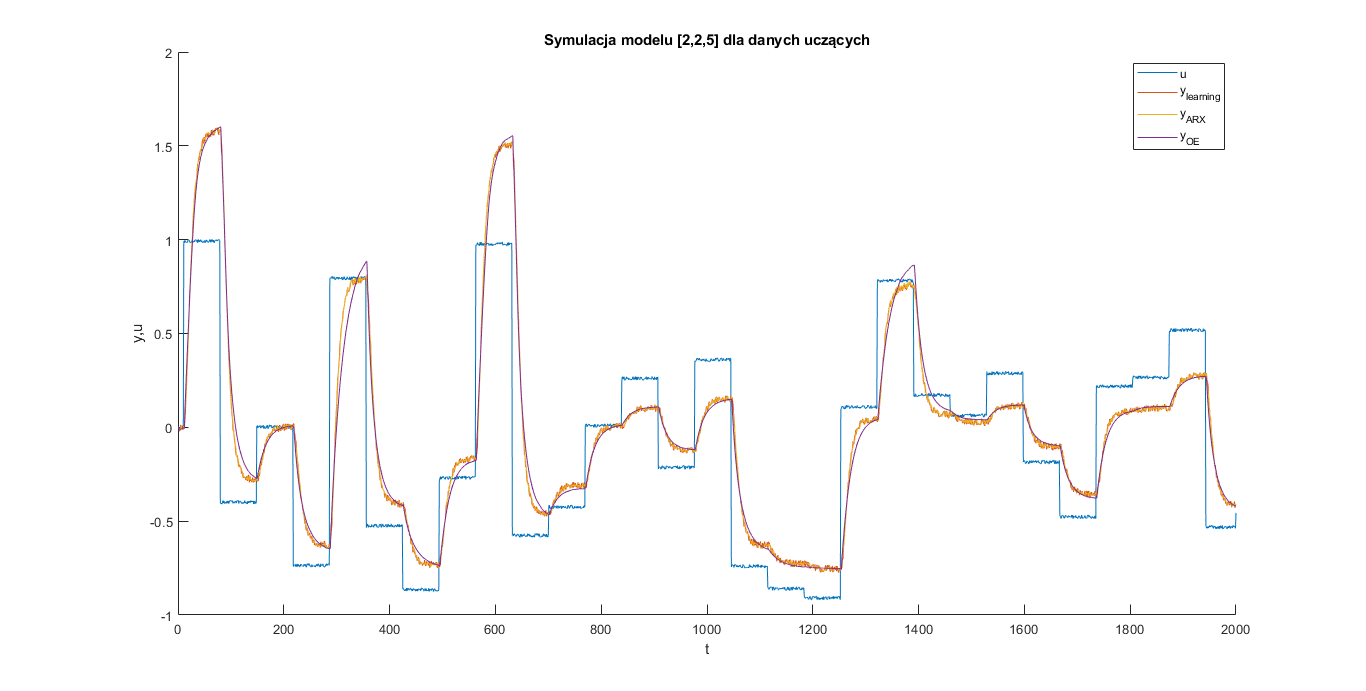
\includegraphics[width=16cm,trim={3cm 0.5cm 3cm 0.5cm},clip]{images/d28.png}
\caption{Działanie modelu dynamicznego o 5. stopniu wielomianu i rzędowi dynamiki 2. dla zbioru uczącego.}
\label{fig:d28}
\end{figure}
\begin{figure}[H]
\centering
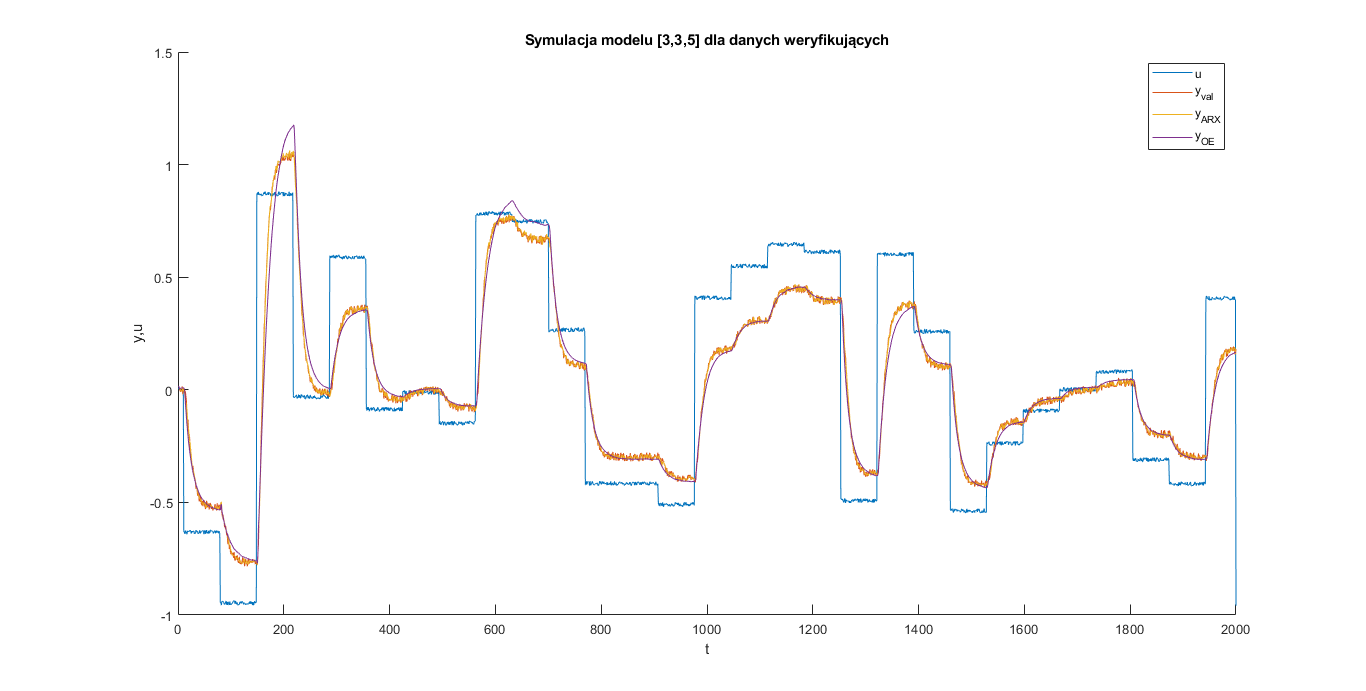
\includegraphics[width=16cm,trim={3cm 0.5cm 3cm 0.5cm},clip]{images/d29.png}
\caption{Działanie modelu dynamicznego o 5. stopniu wielomianu i rzędowi dynamiki 3. dla zbioru weryfikującego.}
\label{fig:d29}
\end{figure}
\begin{figure}[H]
\centering
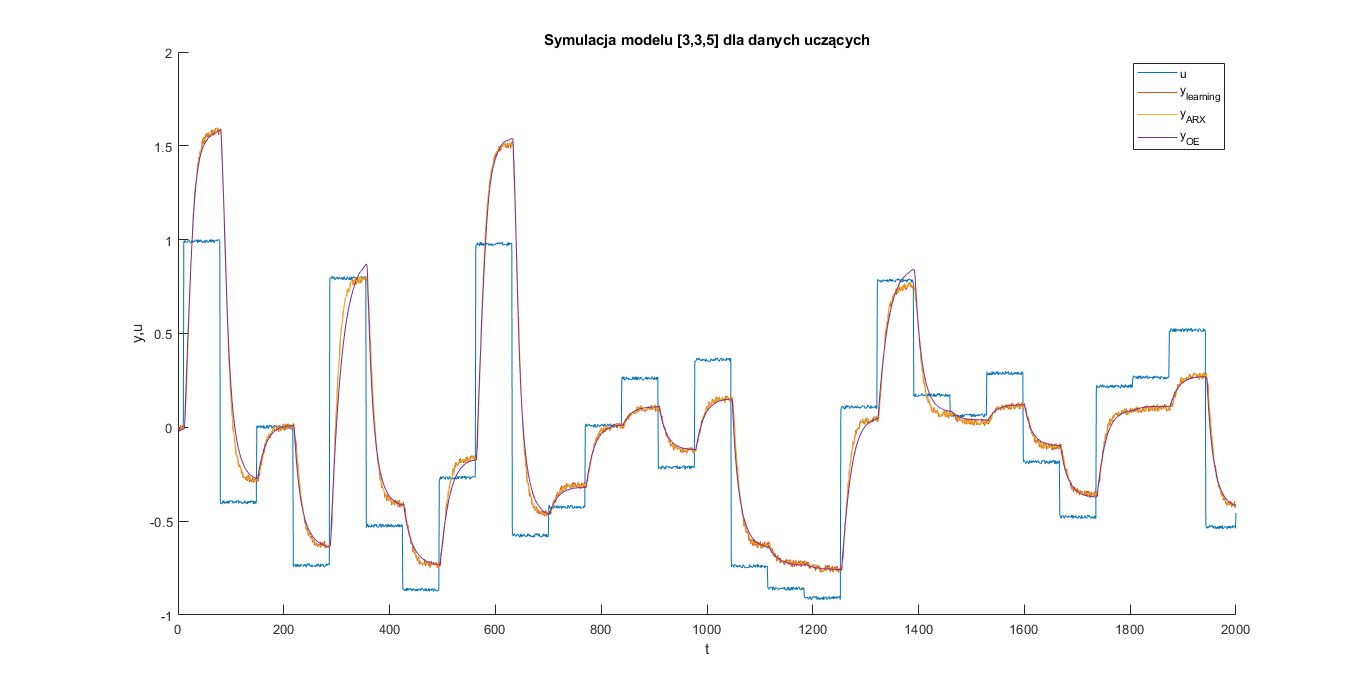
\includegraphics[width=16cm,trim={3cm 0.5cm 3cm 0.5cm},clip]{images/d30.png}
\caption{Działanie modelu dynamicznego o 5. stopniu wielomianu i rzędowi dynamiki 3. dla zbioru uczącego.}
\label{fig:d30}
\end{figure}
\subsection{Podsumowanie}
Jako najlepszy model dynamiczny został wybrany model z dynamiką 3. rzędu oraz wielomianem 4. stopnia. Jak widać na wykresie przedstawiającym błędy poszczególnych modeli, w szczególności w trybie rekurencyjnym, modele z wielomianem o 4. stopniu cechują się najmniejszą wartością błędu, to znaczy, że modele o wyższych stopniach są przewymiarowane i zbyt dopasowane do danych uczących. Dlatego właśnie przy wyborze najlepszego modelu, pod uwagę brano modele właśnie 4. stopnia. \\
Zwiększanie rzędu modelu natomiast powoduje nieznaczne zmiejszanie wartości błędu. Biorąc pod uwagę fakt, żeby ograniczyć ilość parametrów modelu, na podstawie wizualnej oceny przebiegów wybrano model o dynamice 3. rzędu.
\newpage
\section{Charakterystyka statyczna na podstawie modelu dynamicznego}
Charakterystykę statyczną na podstawie modelu dynamicznego czwartego stopnia i dynamice trzeciego rzędu wyznaczono obliczając dla kolejnych wartoścu sterowania z przedziału <-1:1> wartość y spełniającą równanie:
\begin{equation}
y - y_mod = y - f(u,u,u,y,y,y)=0
\end{equation}
ponieważ w stanie statycznym wartość sygnału sterowania oraz wyjście modelu mają stałą wartość.
\begin{equation}
u(k-1)=u(k-2)=u(k-3)=u
\end{equation}
\begin{equation}
y(k-1)=y(k-2)=y(k-3)=y
\end{equation}
Równanie to rozwiązano przy użyciu solvera $fsolve$ programu Matlab. Jest to solver iteracyjny, wymaga więc określenia punktu poczatkowego rozwiązania. Obliczenia powtórzono dla róznych punktów początkowych z przedziału <-1,1>, za kazdym razem otrzymując identyczną charakterystykę. Przedstawiono ją na poniższym wykresie, ą porównując ją jednocześnie z charakterystyką modelu statycznego z zadania 1.
\begin{figure}[H]
\centering
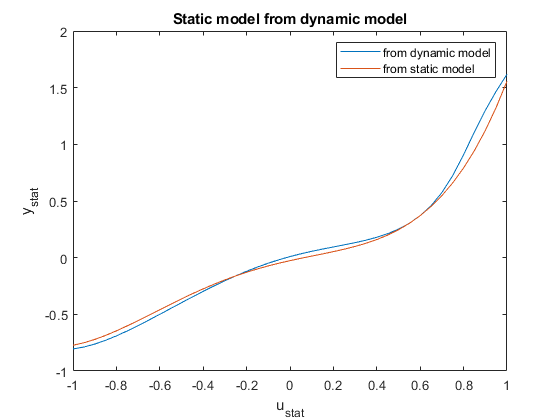
\includegraphics[width=15cm]{images/static_dynamic.png}
\caption{Porównanie modelu statycznego z ch. statyczną wyznaczoną z modelu dynamicznego.}
\label{fig:static_dynamic}
\end{figure}
Jak widać, otrzymane charakterystyki są do siebie zbliżone. \\
Następnie, eksperymentalnie wyznaczono cztery wartości statyczne przy użyciu tego samego modelu dynamicznego. Dla zadanych wartości $u_{0}$, wykonano symulację skoku z wartości 0 do $u_{0}$ na horyzoncie symulacji wielokrotnie dłuższym niż horyzont dynamiki modelowanego obiektu. Wartości otrzymane pod koniec symulacji są wartościami statycznymi $y_{0}$. Otrzymane w ten sposób punkty porównano z charakterystyką wyznaczoną w sposób numeryczny.
\begin{figure}[H]
\centering
\includegraphics[width=15cm]{images/static_dynamic_vs_experiment.png}
\caption{Ch.statyczna z modelu dynamicznego vs. eksperymentalne wartości statyczne}
\label{fig:static_dynamic_vs_experiment}
\end{figure}
Widać, że otrzymane eksperymentalnie wartości statyczne są zgodne z wyznaczoną wcześniej charakterystyką.
\subsection{Wnioski}
\begin{itemize}
\item model dynamiczny (a więc i dane przedstawiające pracę dynamiczną obiektu) może posłużyć również do wyznaczenia modelu statycznego. Jest to szczególnie przydatne, kiedy nie możemy bezpośrednio przeprowadzić eksperymentu wyznaczającego kolejne wartości statyczne obiektu (np. z powodu czasu, jaki jest potrzebny do ustalenia się wartości wyjściowych).
\item ''model statyczny'' otrzymany przy użyciu modelu dynamicznego i solvera jest stosunkowo szybki, kiedy wykorzystuje jako punkt początkowy poprzednią wyliczoną wartość y - potrzebuje on pojedynczych iteracji do znalezienia rozwiązania, często tylko jedną. Mógłby być wykorzystywany w systemach czasu rzeczywistego.
\end{itemize}